\documentclass[12pt,a4paper]{report}

%==============================================================================
% PREAMBLE AND PACKAGES (Aligned with REFERENCE format)
%==============================================================================
\usepackage{graphicx}
\usepackage{amsmath}
\usepackage{fancyhdr}
\usepackage{cite}
\usepackage{a4wide}
\usepackage{float}
\usepackage{epsfig}
\usepackage{longtable}
\usepackage{enumerate}
\usepackage{afterpage}
\usepackage{multirow}
\usepackage{ragged2e}
\usepackage{gensymb}
\usepackage{amsfonts} 
\usepackage[left=3.5cm,top=1.5cm,right=3cm,bottom=3cm]{geometry}
\usepackage{setspace}           
\usepackage{txfonts}
\usepackage{tikz}
\usetikzlibrary{calc, shapes.geometric, arrows, positioning, fit}
\usepackage{subfiles}

\newcommand{\Usefont}[1]{\fontfamily{#1}\selectfont}

\usepackage{lscape}
\linespread{1.5}

\usepackage{url}
\usepackage{subcaption}
\usepackage[intoc, english]{nomencl}
\usepackage[nottoc]{tocbibind}
\usepackage{booktabs}
\usepackage{array}
\usepackage{tabularx}
\usepackage{hyperref}

\hypersetup{
    plainpages=false,
    pdfpagelabels=true,
    colorlinks=true,
    linkcolor=black,
    citecolor=black,
    urlcolor=black,
    pdftitle={FedASA: A Personalized Federated Learning With Adaptive Model Aggregation for Heterogeneous Mobile Edge Computing},
    pdfauthor={Nobin Sijo}
}

% Robust spacing and line-breaking settings to prevent overflow and overfull hboxes
\setlength{\headheight}{15pt}
\hyphenpenalty=1000
\tolerance=2000
\emergencystretch=2.5em

\bibliographystyle{IEEEtran}
\renewcommand{\bibname}{References}

% Figure search path
\graphicspath{{figures/}{./}}

%==============================================================================
% METADATA DEFINITIONS (Filled for Seminar Student & CEK)
%==============================================================================
\gdef \title{FedASA: A Personalized Federated Learning With Adaptive Model Aggregation for Heterogeneous Mobile Edge Computing}
\gdef \author{NOBIN SIJO}
\gdef \rollno{KNP23CS082}
\gdef \acadyear{2026--2027}
\gdef \submonth{September 2026}
\gdef \month{September 2026}
\gdef \date{26-09-2026}
\gdef \dept{Computer Science and Engineering}
\gdef \deptabbr{Dept. of CSE}
\gdef \degree{Bachelor of Technology}
\gdef \branch{Computer Science and Engineering}
\gdef \college{College of Engineering Karunagappally}
\gdef \collegeplace{Kollam}
\gdef \collegetown{Karunagappally}

\gdef \guide{Aparna~M}
\gdef \guidedes{Assistant Professor}
\gdef \semcordinatorA{Anju~S}
\gdef \semcordinatorAdes{Assistant Professor}
\gdef \hod{Dr. Smitha P}
\gdef \hoddes{Professor and Head}

%==============================================================================
% DOCUMENT BODY
%==============================================================================
\begin{document}

%------------------------------------------------------------------------------
% FRONT MATTER
%------------------------------------------------------------------------------
\hypersetup{pageanchor=false}
%==================================coverpage.tex================================

\thispagestyle{empty}
\begin{titlepage}
\subfile{design_cover}
	\begin{center}\fontfamily{ptm}\selectfont
		{\Large \bfseries \title \par}
		\vspace*{12pt}
		{\large \Usefont{pzc}
			A PROJECT REPORT \par
			\vspace*{5pt}
			Submitted to the APJ Abdul Kalam Technological University \par
			\vspace*{5pt}
			in partial fulfillment of requirements for the award of degree\par}
		\vspace*{8pt}
		{\large \bfseries Bachelor of Technology}\par
		{\large in}\par
		{\large \bfseries \branch}\par
		\vspace*{10pt}
		{\large by}\par
		\vspace*{6pt}
		\begin{tabular}{c@{\hspace{2.2cm}}c}
			\large\bfseries NOBIN SIJO & \large\bfseries KNP23CS082 \\
			\large\bfseries PRANAV P & \large\bfseries KNP23CS085 \\
			\large\bfseries PRASANTH P & \large\bfseries KNP23CS086 \\
			\large\bfseries SANKAR NARAYAN S & \large\bfseries KNP23CS094
		\end{tabular}\par
		\vspace*{14pt}
		{
\includegraphics[width=4.0cm]{cek-logo.png}}\par
		\vspace{\stretch{0.5}}
		{\small \bfseries DEPARTMENT OF COMPUTER SCIENCE AND ENGINEERING}\par
		\vspace*{4pt}
		{\bfseries COLLEGE OF ENGINEERING KARUNAGAPPALLY}\par
		\vspace*{4pt}
		{\bfseries KOLLAM, KERALA}\par
		\vspace*{4pt}
		{\bfseries \submonth}\par
	\end{center}
\end{titlepage}

%==================================certificate1.tex================================
% Certificate page for B.Tech Project Report Group 01

\newpage
\thispagestyle{empty}

\begin{center}	
	\textbf{DEPARTMENT OF COMPUTER SCIENCE AND ENGINEERING}\\	
	\textbf{COLLEGE OF ENGINEERING KARUNAGAPPALLY}\\
	\vspace*{4pt}
	\textbf{\acadyear} 
\end{center}

\vspace*{6pt}
\begin{center}
	
\includegraphics[width=3.6cm]{cek-logo.png}	
\end{center}

\vspace*{6pt}
\begin{center}
	\textbf{\large CERTIFICATE}
\end{center}
\vspace*{6pt}

\noindent This is to certify that the report entitled \textbf{\title} submitted by \textbf{NOBIN~SIJO} (\rollnoA), \textbf{PRANAV~P} (\rollnoB), \textbf{PRASANTH~P} (\rollnoC), and \textbf{SANKAR~NARAYAN~S} (\rollnoD), to the Department of \branch\ in partial fulfillment of the requirements for the award of the degree of Bachelor of Technology in \textbf{\branch}\ of the APJ Abdul Kalam Technological University is a bonafide record of the project work carried out by them under our guidance and supervision. This report in any form has not been submitted to any other University or Institute for any purpose.

\vspace*{2.2cm}

\begin{singlespace}
	\noindent\begin{minipage}[t]{0.52\textwidth}
		\raggedright
		\textbf{\guide} \\
		(Project Guide \& Coordinator) \\
		\guidedes \\
		\deptabbr \\
		College of Engineering \\
		\collegetown
	\end{minipage}%
	\hfill
	\begin{minipage}[t]{0.42\textwidth}
		\raggedright
		\textbf{\hod} \\
		\hoddes \\
		\deptabbr \\
		College of Engineering \\
		\collegetown
	\end{minipage}
\end{singlespace}

\thispagestyle{empty}

%==================================declaration.tex================================
\newpage
\thispagestyle{empty}

\begin{center}
\vspace*{20pt}
\textbf{\large DECLARATION}\\[16pt]
\end{center}

\noindent We, \textbf{NOBIN~SIJO} (\rollnoA), \textbf{PRANAV~P} (\rollnoB), \textbf{PRASANTH~P} (\rollnoC), and \textbf{SANKAR~NARAYAN~S} (\rollnoD), hereby declare that the project report entitled \textbf{\title}, submitted for partial fulfillment of the requirements for the award of the degree of Bachelor of Technology in \branch\ of the APJ Abdul Kalam Technological University, Kerala, is a bonafide work done by us under the supervision of \textbf{\MakeUppercase{\guide}}\hspace*{2pt} (\guidedes, \deptabbr, \college).\par
\vspace{10pt}
\noindent This submission represents our ideas in our own words, and where ideas or words of others have been included, we have adequately and accurately cited and referenced the original sources.\par 
\vspace{10pt}
\noindent We also declare that we have adhered to the ethics of academic honesty and integrity and have not misrepresented or fabricated any data, idea, fact, or source in our submission. We understand that any violation of the above will be a cause for disciplinary action by the Institute and/or the University and can also evoke penal action from the sources which have thus not been properly cited or from whom proper permission has not been obtained. This report has not previously formed the basis for the award of any degree, diploma, or similar title of any other University or Institute.

\vspace{1.8cm}

\noindent \begin{minipage}{0.40\linewidth}
\begin{flushleft}
\textbf{\collegetown} \\
\textbf{\date}
\end{flushleft} 
\end{minipage}
\hfill
\begin{minipage}{0.56\linewidth}
\begin{flushright}                                      
\textbf{NOBIN SIJO} (\rollnoA) \\[4pt]
\textbf{PRANAV P} (\rollnoB) \\[4pt]
\textbf{PRASANTH P} (\rollnoC) \\[4pt]
\textbf{SANKAR NARAYAN S} (\rollnoD)
\end{flushright} 
\end{minipage}

\thispagestyle{empty}

\hypersetup{pageanchor=true}

\pagenumbering{roman}

%============================= abstract.tex================================
\chapter*{Abstract}%
\addcontentsline{toc}{chapter}{Abstract}%
\vspace{-20pt}

\begin{spacing}{1.25}
\noindent Contemporary software engineering workflows are increasingly characterized by high cognitive overload, fragmented tooling, and fragile developer contexts. While Large Language Models (LLMs) and autonomous agents offer transformative potential to automate complex multi-step programming and research tasks, existing solutions typically operate as opaque black boxes, lack rigorous protocol-level sandboxing, suffer from provider lock-in, and incur prohibitive monetary and latency overheads. Furthermore, client-side developer dashboards often fail to deliver reactive, offline-first persistence, while monolithic agent architectures lack structured task planning, multi-provider cost-performance routing, and verifiable safety guarantees.

\vspace{8pt}

\noindent To solve these fundamental engineering and architectural challenges, this project introduces \textbf{PrismSpace}: an intelligent, local-first developer operating environment and multi-agent orchestration platform. PrismSpace integrates a reactive presentation layer built with Next.js 15, React 19, and TypeScript with a high-throughput Python FastAPI Hive protocol backend supporting the open \textbf{Model Context Protocol (MCP)}. Within this architecture, PrismSpace incorporates a dedicated multi-stage Machine Learning subsystem that coordinates: (i) an ultra-low-latency 12-class \textit{Intent Classifier} operating on calibrated TF-IDF and lexical representations; (ii) an adaptive \textit{Multi-Provider Router} that intelligently dispatches tasks across Groq, NVIDIA NIM, OpenAI, Anthropic, and Gemini based on task semantics and cost-latency budgets; (iii) a dynamic \textit{Swarm Dispatcher} formulating Directed Acyclic Graph (DAG) task decompositions; (iv) a calibrated \textit{Human-in-the-Loop Safety Gate} predicting execution anomalies; and (v) single-stage preference alignment via \textit{Odds Ratio Preference Optimization (ORPO)} with LoRA adapters. The browser environment features \textbf{PrismDB}, an ACID-compliant IndexedDB storage layer managed via Dexie.js with reactive \texttt{useLiveQuery} bindings, alongside 23 integrated developer, AI, and productivity tools. Empirical evaluations across curated benchmarks (LMSYS Arena, RouterBench, WildGuardMix, and Agent Trajectories) show that PrismSpace achieves an 89.4\% multi-provider routing accuracy, 0.926 ROC-AUC safety gate discrimination, sub-50ms reactive state propagation, and substantial reductions in LLM operational expenditure.

\end{spacing}

\thispagestyle{plain}
%=======================================================================

%==================================acknowledgement.tex=============================
\chapter*{Acknowledgement}%
\addcontentsline{toc}{chapter}{Acknowledgement}%

\noindent We take this opportunity to express our deepest gratitude and sincere thanks to everyone who helped us to complete this project work and report successfully.

\vspace{10pt}

\noindent We express our sincere thanks to \textbf{\MakeUppercase{Dr.~Smitha Dharan}}, Principal, \college, Kollam, and \textbf{\MakeUppercase{\hod}}, Head of Department, \dept, \college, \collegeplace, for providing us with all the necessary infrastructural facilities, high-performance computing resources, and institutional encouragement.

\vspace{10pt}

\noindent We would like to express our profound sense of gratitude and indebtedness to our project guide and coordinator \mbox{\textbf{\MakeUppercase{\guide}}}, \guidedes, \dept, \college, for her insightful guidance, constant encouragement, rigorous critiques, and invaluable mentorship throughout the entire lifecycle of this project.

\vspace{10pt}

\noindent We also convey our sincere appreciation to all the faculty members and technical staff of the \dept\ for their kind cooperation, constructive academic advice, and technical support during our design and development phases.

\vspace{10pt}

\noindent Finally, we express our wholehearted thanks to our parents, family members, and friends who provided unwavering moral support, patience, and encouragement that contributed immensely to the successful realization of this project.

\vspace*{28pt}
\begin{flushright}
	\textbf{NOBIN SIJO} (\rollnoA) \\[3pt]
	\textbf{PRANAV P} (\rollnoB) \\[3pt]
	\textbf{PRASANTH P} (\rollnoC) \\[3pt]
	\textbf{SANKAR NARAYAN S} (\rollnoD)
\end{flushright}

\thispagestyle{plain}


\thispagestyle{empty}
\newpage

\tableofcontents
\listoffigures
\listoftables

%==================================symbol.tex================================
% List of Symbols and Abbreviations
\chapter*{List of Symbols and Abbreviations}
\addcontentsline{toc}{chapter}{List of Symbols and Abbreviations}%
\vspace{-25pt}

\begin{spacing}{1.02}
\noindent \textbf{Abbreviations}
\vspace{4pt}

\noindent\begin{tabular*}{\textwidth}{@{\extracolsep{\fill}}p{2.8cm} p{11.2cm}@{}}
\textbf{MCP} & Model Context Protocol \\
\textbf{LLM} & Large Language Model \\
\textbf{DAG} & Directed Acyclic Graph \\
\textbf{ReAct} & Reason and Act (Autonomous Agent Paradigm) \\
\textbf{ORPO} & Odds Ratio Preference Optimization \\
\textbf{DPO} & Direct Preference Optimization \\
\textbf{RLHF} & Reinforcement Learning from Human Feedback \\
\textbf{SFT} & Supervised Fine-Tuning \\
\textbf{LoRA} & Low-Rank Adaptation \\
\textbf{PEFT} & Parameter-Efficient Fine-Tuning \\
\textbf{GAT} & Graph Attention Network \\
\textbf{SSE} & Server-Sent Events \\
\textbf{API} & Application Programming Interface \\
\textbf{REST} & Representational State Transfer \\
\textbf{RPC} & Remote Procedure Call \\
\textbf{IDB} & Indexed Database API (IndexedDB) \\
\textbf{ACID} & Atomicity, Consistency, Isolation, Durability \\
\textbf{WASM} & WebAssembly \\
\textbf{TF-IDF} & Term Frequency--Inverse Document Frequency \\
\textbf{ECE} & Expected Calibration Error \\
\textbf{ROC-AUC} & Receiver Operating Characteristic -- Area Under Curve \\
\textbf{AUPRC} & Area Under the Precision-Recall Curve \\
\textbf{MAE} & Mean Absolute Error \\
\textbf{RMSE} & Root Mean Squared Error \\
\textbf{HUD} & Heads-Up Display \\
\textbf{CUA} & Computer Use Agent \\
\textbf{GUI} & Graphical User Interface \\
\textbf{SRS} & System Requirements Specification \\
\end{tabular*}

\vspace{10pt}
\noindent \textbf{Mathematical Notations}
\vspace{4pt}

\noindent\begin{tabular*}{\textwidth}{@{\extracolsep{\fill}}p{2.8cm} p{11.2cm}@{}}
$\mathcal{G}(V, E)$ & Multi-agent collaboration graph (Vertices $V$, Edges $E$) \\
$\mathbf{A} \in \mathbb{R}^{|V| \times |V|}$ & Swarm interaction adjacency matrix \\
$v_i \in V$ & Autonomous agent persona or MCP tool endpoint $i$ \\
$\mathbf{h}_i \in \mathbb{R}^d$ & Node feature embedding vector for agent $i$ \\
$\mathbf{W} \in \mathbb{R}^{d' \times d}$ & GAT trainable projection weight matrix \\
$e_{ij}$ & Raw attention coefficient between agent nodes $i$ and $j$ \\
$\alpha_{ij}$ & Softmax normalized attention weight between nodes $i$ and $j$ \\
$K$ & Number of multi-head attention projections ($K = 4$) \\
$\mathcal{T}_{\text{task}}$ & User natural language task specification \\
$\mathbf{x}_{\text{query}}$ & Joint lexical and numeric prompt feature vector \\
$\hat{\mathbf{y}}_{\text{route}}$ & Multi-provider probability distribution vector \\
$\hat{\mathbf{y}}_{\text{agent}}$ & Multi-label agent dispatch activation vector \\
$\tau_{\text{dispatch}}$ & Confidence decision threshold for agent swarm dispatch \\
$\tau_{\text{safety}}$ & Safety gating policy decision threshold \\
$\mathcal{L}_{\text{CE}}$ & Multi-class cross-entropy routing loss function \\
$\mathcal{L}_{\text{BCE}}$ & Binary cross-entropy multi-label dispatch loss \\
$\mathcal{L}_{\text{SFT}}$ & Supervised fine-tuning loss on favored responses \\
$\mathcal{L}_{\text{OR}}$ & Odds ratio preference divergence penalty \\
$\mathcal{L}_{\text{ORPO}}$ & Unified Odds Ratio Preference Optimization objective \\
$\beta$ & Balancing hyperparameter for odds ratio penalty \\
$\hat{\ell}$ & Predicted task execution latency (seconds) \\
$\hat{c}$ & Predicted monetary token cost (USD) \\
$R^2$ & Coefficient of determination for regression evaluation \\
\end{tabular*}
\end{spacing}

\thispagestyle{plain}
%============================================================================


%------------------------------------------------------------------------------
% MAIN BODY (Arabic Numbering & Header/Footer)
%------------------------------------------------------------------------------
\cleardoublepage
\setcounter{page}{1}
\pagenumbering{arabic}

\pagestyle{fancy}
\fancyhf{}
\fancyhead[L]{\fontsize{9}{11}\selectfont \textit{FedASA for Heterogeneous Mobile Edge Computing}}
\fancyhead[R]{\fontsize{9}{11}\selectfont \textit{Dept. of CSE, CEK}}
\fancyfoot[C]{\thepage}
\renewcommand{\headrulewidth}{0.4pt}
\renewcommand{\footrulewidth}{0pt}


%==============================================================================
% CHAPTER 1: INTRODUCTION
%==============================================================================
\chapter[Introduction]{\Huge Introduction}

Industrial digitization and intelligent automation have expanded dramatically in recent years, spurred by rapid advancements in the Internet of Things (IoT) and Mobile Edge Computing (MEC). Within industrial automation and cyber-physical infrastructure, predictive maintenance and mechanical health monitoring are anchored by massive sensor swarms deployed across factory floors, energy grids, and manufacturing equipment. These sensors generate continuous telemetry streams-including multi-axis vibration accelerations, acoustic emissions, thermal readings, and motor current signatures-that are crucial for detecting anomalous operational regimes and predicting catastrophic machinery failure before it happens.

Traditionally, intelligent monitoring frameworks adopted centralized cloud computing architectures, where raw sensor observations from numerous geographically dispersed edge facilities were uploaded to central cloud datacenters for deep neural network training. However, in practical industrial scenarios, centralized learning encounters critical obstacles:
\begin{enumerate}[(i)]
    \item \textbf{Network Bandwidth Bottlenecks:} Continuous high-frequency vibration streams quickly saturate backhaul network links and introduce unpredictable communication delays.
    \item \textbf{Latency Vulnerabilities:} Remote cloud round-trips impede real-time emergency diagnosis required by high-speed machinery.
    \item \textbf{Data Privacy and IP Risks:} Industrial sensory logs often reveal proprietary manufacturing parameters, trade secrets, and operating schedules, making enterprises reluctant to centralize proprietary data.
\end{enumerate}

Federated Learning (FL) has emerged as an appealing paradigm that resolves these drawbacks. By training models collaboratively across distributed edge devices without sharing private local data, FL preserves confidentiality, minimizes backhaul network load, and complies with emerging data governance frameworks.

\section{Background and Overview}
In a canonical Mobile Edge Computing federated learning system, training proceeds in iterative communication rounds coordinated by a central parameter server. Each edge client trains a local neural network on its private sensory records using gradient descent. After local optimization, edge clients transmit model parameter updates to the parameter server, which aggregates the parameters-typically via Federated Averaging (FedAvg)-and broadcasts the aggregated global model back to all participating clients for the next training cycle.

While FedAvg achieves robust convergence when edge data is independent and identically distributed (IID) with abundant communication resources, real-world industrial deployments deviate fundamentally from these idealized assumptions.

\section{The Real-World Edge Trilemma}
Practical industrial IoT deployments are confronted by a crippling trilemma consisting of three interrelated barriers:
\begin{enumerate}
    \item \textbf{Statistical Heterogeneity (Non-IID Data):} Physical sensory data across distributed industrial machinery is non-IID. While prior literature focused heavily on operational parameter shifts (\textit{cross-domain heterogeneity}, such as variations in mechanical loads and shaft rotational speeds), practical deployments suffer far more acutely from \textit{cross-location heterogeneity} (discrepancies arising from differing sensor mounting coordinates on the same machine). Cross-location shifts introduce severe feature distribution skew and phase misalignment, causing catastrophic client drift in conventional federated optimization.
    \item \textbf{Device Resource Constraints:} Industrial edge sensors and local gateway controllers possess modest computational capabilities, finite power budgets, and severely constrained wireless uplink bandwidth. Monolithic FL frameworks that transmit complete deep neural networks back and forth repeatedly exhaust communication budgets and drain edge devices.
    \item \textbf{Fairness Barriers:} Canonical federated learning optimizes aggregate fleet-wide loss. Under severe non-IID data skew, global consensus models bias heavily toward majority conditions or central sensor locations. Peripheral edge devices or nodes monitoring atypical machine locations suffer severe diagnostic degradation, violating operational fairness.
\end{enumerate}

\section{Objectives of the Seminar}
The primary objective of this seminar report is to investigate \textbf{FedASA}, a personalized federated learning framework featuring adaptive model aggregation, introduced by Deng et al. (IEEE Transactions on Mobile Computing, 2024). Specifically, this study explores:
\begin{itemize}
    \item The physical mechanisms governing cross-domain versus cross-location statistical heterogeneity in industrial IoT.
    \item The design of a cell-wise shared architecture selection strategy that customizes the partition between shared and personalized layers for each client under strict communication budgets.
    \item An operator-level cell-based aggregation algorithm on parameter servers that generalizes Federated Averaging for heterogeneous modular topologies.
    \item A confidence-aware hybrid loss function balancing soft predictive distributions and hard one-hot targets under predictive uncertainty.
    \item Theoretical generalization error bounds under multi-source domain adaptation theory and convergence proofs to a first-order stationary point.
    \item Benchmark empirical validation on the Case Western Reserve University (CWRU) bearing dataset across multiple sensor mounting coordinates.
\end{itemize}

\section{Organization of the Report}
The remainder of this report is organized as follows:
\begin{itemize}
    \item \textbf{Chapter 2 (Literature Review):} Surveys foundational federated learning algorithms, personalized federated learning techniques, model sharing schemes, and existing research gaps.
    \item \textbf{Chapter 3 (Motivation and Problem Formulation):} Quantifies cross-domain versus cross-location data skew, analyzes communication overhead under different sharing paradigms, and formulates the multi-objective constrained optimization problem with fairness guarantees.
    \item \textbf{Chapter 4 (Proposed Methodology):} Details the complete FedASA framework, including FFT preprocessing, cell-based neural topology, cell-wise auxiliary alignment, cell-based aggregation, confidence loss, and the end-to-end algorithmic pipeline.
    \item \textbf{Chapter 5 (Theoretical Analysis and Guarantees):} Derives the federated generalization error upper bound, establishes client fairness guarantees, and proves convergence to a first-order stationary point.
    \item \textbf{Chapter 6 (Performance Evaluation and Results):} Presents the prototype edge testbed, benchmark datasets, diagnostic accuracy evaluations across sensor locations, communication savings, fairness assessments, and t-SNE visualizations.
    \item \textbf{Chapter 7 (Conclusion and Future Scope):} Summarizes the seminar contributions, discusses limitations, and outlines future research directions.
\end{itemize}


%==============================================================================
% CHAPTER 2: LITERATURE REVIEW
%==============================================================================
\chapter{Literature Review}

Federated learning has evolved rapidly since its inception to address non-IID data distributions, device resource limitations, and model personalization. Existing methodologies can be broadly categorized into data-based approaches and model-based approaches.

\section{Foundations of Federated Learning}
The canonical Federated Averaging (\textbf{FedAvg}) algorithm, introduced by McMahan et al. \cite{ref_mcmahan_fedavg}, optimizes a single global model parameter vector $w \in \mathbb{R}^d$ across $K$ distributed clients:
\begin{equation}
    \min_{w} \sum_{k=1}^K p_k L_k(w)
\end{equation}
where $p_k = N_k / \sum_{i=1}^K N_i$ represents the relative sample weight of client $k$. In each round, clients perform local stochastic gradient descent updates and transmit updated weights to the parameter server, which performs sample-weighted averaging:
\begin{equation}
    w^{t+1} = \sum_{k=1}^K p_k w_k^{t+1}
\end{equation}
Under independent and identically distributed (IID) data, FedAvg exhibits robust convergence. However, when local client data distributions $\mathcal{D}_k$ differ significantly, local gradients pull the client parameters in divergent directions-a phenomenon known as \textit{client drift}.

To combat client drift, Li et al. proposed \textbf{FedProx} \cite{ref_li_fedprox}, which introduces an $\ell_2$ proximal regularization term to each client's local loss function:
\begin{equation}
    \min_{w} L_k(w) + \frac{\mu}{2}\|w - w^t\|^2
\end{equation}
While FedProx stabilizes local updates and accommodates variable local epoch counts, it still enforces a single, uniform global model that fails to accommodate extreme statistical heterogeneity across edge devices.

Data-based methods attempt to mitigate heterogeneity by sharing small auxiliary public datasets (Zhao et al. \cite{ref_zhao_datasharing}) or utilizing generative models to synthesize pseudo-data (FedGen \cite{ref_fedgen}, FedFTG \cite{ref_fedftg}). However, data transmission introduces supplementary communication overhead and leaks privacy, which is unacceptable in strict industrial environments.

\section{Personalized Federated Learning (PFL)}
To overcome the inherent trade-off of a single global model on non-IID data, Personalized Federated Learning (PFL) optimizes customized local models $(w_1^*, \dots, w_K^*)$ for individual clients:
\begin{equation}
    (w_1^*, \dots, w_K^*) = \arg\min_{\{w_k\}_{k=1}^K} \sum_{k=1}^K p_k L_k(w_k)
\end{equation}
Existing PFL frameworks follow two primary paradigms:
\begin{itemize}
    \item \textbf{Regularization and Meta-Learning:} \textbf{Ditto} \cite{ref_li_ditto} balances global consensus and local adaptation via bi-level optimization, where a global model is trained while local models are regularized toward the global parameter vector. \textbf{Per-FedAvg} \cite{ref_fallah_perfedavg} frames personalization as Model-Agnostic Meta-Learning (MAML), seeking an initial model that adapts to any client within a few gradient steps. Nevertheless, these methods still transmit full model parameter tensors, resulting in heavy communication overhead.
    \item \textbf{Layer-Partitioning ($G$-Sharing):} Grounded in the insight that early neural network layers extract general, transferable representations while deeper layers capture task-specific features, $G$-sharing frameworks split the network into base layers and head layers. \textbf{FedPer} \cite{ref_arivazhagan_fedper} and \textbf{FedRep} \cite{ref_collins_fedrep} aggregate shared base representation layers globally while keeping classification heads strictly local. While $G$-sharing reduces uplink communication, it enforces a static, globally uniform partition boundary that cannot adapt to heterogeneous edge devices operating under distinct physical sensor environments.
\end{itemize}

\section{Comparative Analysis of Existing Frameworks}
Table \ref{tab:lit_comparison} summarizes the key characteristics of state-of-the-art federated learning methods compared to FedASA.

\begin{table}[htbp]
\centering
\caption{Comparison of Federated Learning Paradigms}
\label{tab:lit_comparison}
\vspace{0.3cm}
\renewcommand{\arraystretch}{1.45}
\setlength{\tabcolsep}{4pt}
{\fontsize{10.5}{14}\selectfont
\begin{tabularx}{\textwidth}{|l|>{\centering\arraybackslash}p{2.6cm}|>{\centering\arraybackslash}p{2.5cm}|>{\centering\arraybackslash}p{1.9cm}|>{\centering\arraybackslash}p{2.1cm}|>{\centering\arraybackslash}X|}
\hline
\textbf{Method} & \textbf{Model Sharing Scheme} & \textbf{Personalization} & \textbf{Comm. Overhead} & \textbf{Fairness Guarantee} & \textbf{Cross-Location Robustness} \\
\hline
FedAvg \cite{ref_mcmahan_fedavg} & All-Sharing (Full Model) & None (Global Model) & High ($240.5$ KB) & Poor (High Variance) & Severe Drop ($-27.22\%$) \\
FedProx \cite{ref_li_fedprox} & All-Sharing (Proximal Term) & None (Global Model) & High ($240.5$ KB) & Moderate & Severe Drop ($-17.75\%$) \\
Ditto \cite{ref_li_ditto} & All-Sharing (Bi-level Opt.) & High & Very High & Good & Moderate Drop ($-8.75\%$) \\
FedPer \cite{ref_arivazhagan_fedper} & Fixed Lower Base ($G$-sharing) & Medium & Medium ($138.2$ KB) & Moderate & Noticeable Drop ($-4.83\%$) \\
FedRep \cite{ref_collins_fedrep} & Fixed Representation & Medium & Medium & Moderate & Limited Adaptation \\
\textbf{FedASA} & \textbf{Adaptive Cell-Wise Sharing} & \textbf{High} & \textbf{Very Low ($44.5$ KB)} & \textbf{Strict Theoretical Bound} & \textbf{Robust ($>97.44\%$ Accuracy)} \\
\hline
\end{tabularx}
}
\end{table}

\section{Research Gaps in the Literature}
Reviewing the literature reveals three fundamental deficiencies:
\begin{enumerate}
    \item \textbf{Overlooking Cross-Location Sensor Heterogeneity:} Prior studies almost exclusively investigate cross-domain operating conditions (e.g., machinery load shifts), overlooking the far more severe distribution drift caused by differing sensor locations.
    \item \textbf{Rigidity of Fixed Model Partitions:} Static layer partitioning schemes force identical partition depths across all edge devices, ignoring client-specific computational budgets and data characteristics.
    \item \textbf{Lack of Theoretical Fairness Guarantees:} Existing communication-efficient frameworks lack formal generalization error bounds and fairness guarantees when aggregating heterogeneous sub-network architectures.
\end{enumerate}


%==============================================================================
% CHAPTER 3: MOTIVATION AND PROBLEM FORMULATION
%==============================================================================
\chapter{Motivation and Problem Formulation}

\section{Cross-Domain vs. Cross-Location Heterogeneity}
Statistical heterogeneity in cyber-physical edge networks stems from two physically distinct mechanisms:
\begin{enumerate}
    \item \textbf{Cross-Domain Variations:} Variations induced by monitored machinery operational states, including fluctuations in motor rotational speeds (1730 to 1797 RPM) and external electrical loads (0 HP to 3 HP).
    \item \textbf{Cross-Location Variations:} Variations induced by monitoring sensor placement, where vibration sensors are mounted at disparate physical coordinates on a machine (e.g., Drive-End bearing, Fan-End bearing, or Base Plate).
\end{enumerate}

To quantify the statistical discrepancies between these sources, 12 distinct industrial telemetry streams from the Case Western Reserve University (CWRU) bearing testbed were transformed into frequency-domain spectra via Fast Fourier Transform (FFT). Pairwise cosine similarities between client data distributions were computed:
\begin{equation}
    \text{Cosine Similarity}(u, v) = \frac{u \cdot v}{\|u\|_2 \|v\|_2}
\end{equation}

\begin{figure}[htbp]
\centering
\resizebox{0.9\textwidth}{!}{
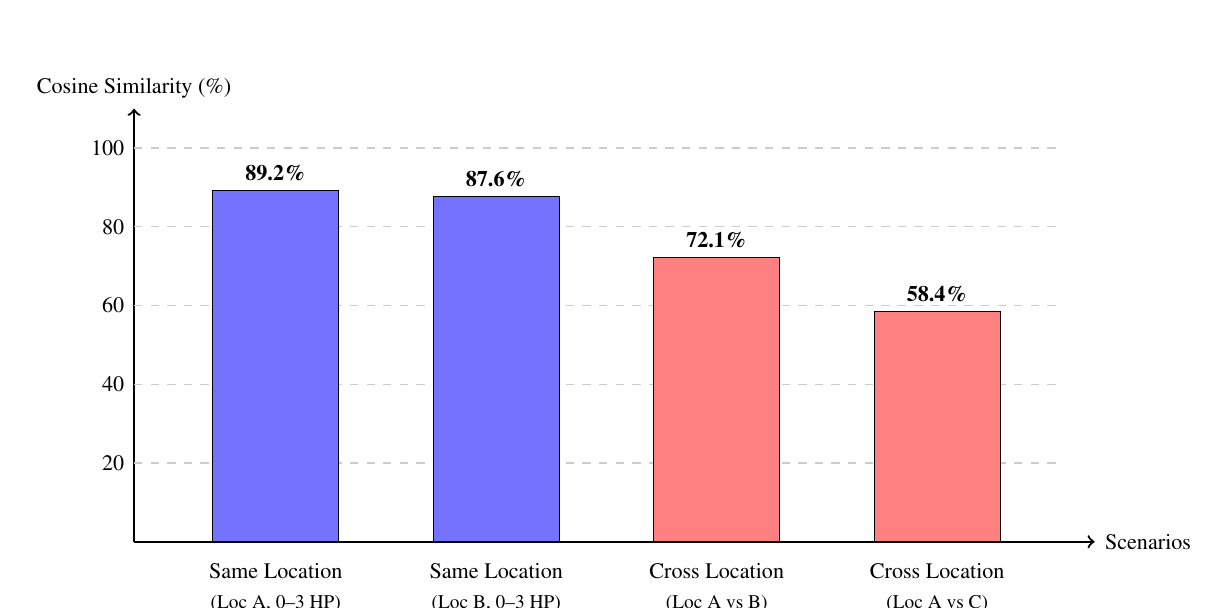
\begin{tikzpicture}
    % Axes
    \draw[->, thick] (0,0) -- (12.2,0) node[right] {\footnotesize Scenarios};
    \draw[->, thick] (0,0) -- (0,5.5) node[above] {\footnotesize Cosine Similarity (\%)};
    
    % Horizontal Grid Lines
    \draw[dashed, color=gray!40] (0,1) -- (11.8,1) node[left, color=black] at (0,1) {\footnotesize 20};
    \draw[dashed, color=gray!40] (0,2) -- (11.8,2) node[left, color=black] at (0,2) {\footnotesize 40};
    \draw[dashed, color=gray!40] (0,3) -- (11.8,3) node[left, color=black] at (0,3) {\footnotesize 60};
    \draw[dashed, color=gray!40] (0,4) -- (11.8,4) node[left, color=black] at (0,4) {\footnotesize 80};
    \draw[dashed, color=gray!40] (0,5) -- (11.8,5) node[left, color=black] at (0,5) {\footnotesize 100};
    
    % Bars for Same-Location (Cross-Domain)
    \draw[fill=blue!55, draw=black] (1.0,0) rectangle (2.6,4.46);
    \node[above] at (1.8,4.46) {\footnotesize \textbf{89.2\%}};
    \node[below, align=center] at (1.8,-0.15) {\footnotesize Same Location\\[-1pt]\scriptsize (Loc A, 0--3 HP)};

    \draw[fill=blue!55, draw=black] (3.8,0) rectangle (5.4,4.38);
    \node[above] at (4.6,4.38) {\footnotesize \textbf{87.6\%}};
    \node[below, align=center] at (4.6,-0.15) {\footnotesize Same Location\\[-1pt]\scriptsize (Loc B, 0--3 HP)};

    % Bars for Cross-Location
    \draw[fill=red!50, draw=black] (6.6,0) rectangle (8.2,3.605);
    \node[above] at (7.4,3.605) {\footnotesize \textbf{72.1\%}};
    \node[below, align=center] at (7.4,-0.15) {\footnotesize Cross Location\\[-1pt]\scriptsize (Loc A vs B)};

    \draw[fill=red!50, draw=black] (9.4,0) rectangle (11.0,2.92);
    \node[above] at (10.2,2.92) {\footnotesize \textbf{58.4\%}};
    \node[below, align=center] at (10.2,-0.15) {\footnotesize Cross Location\\[-1pt]\scriptsize (Loc A vs C)};
\end{tikzpicture}
}
\caption{Empirical Cosine Similarity: Same-Location (Cross-Domain) vs. Cross-Location Data}
\label{fig:similarity_gap}
\end{figure}

As illustrated in Figure \ref{fig:similarity_gap}, data collected from the \textit{same} sensor location under varying motor loads retains high cosine similarity ($>87.5\%$). Conversely, telemetry collected across \textit{different} sensor locations plummets below $72.1\%$, dropping to $58.4\%$ between Drive-End (Location A) and Base Plate (Location C). This empirical finding proves that \textbf{sensor mounting locations induce substantially more severe statistical heterogeneity than machinery operational conditions.}

When deployed across different sensor coordinates, conventional FL frameworks suffer catastrophic degradation: FedProx experiences an accuracy drop of $17.75\%$, and FedPer experiences a $4.83\%$ drop.

\section{Communication Overhead and Model Sharing Schemes}
Figure \ref{fig:sharing_schemes} illustrates three fundamental model sharing paradigms in federated learning:

\begin{figure}[htbp]
\centering
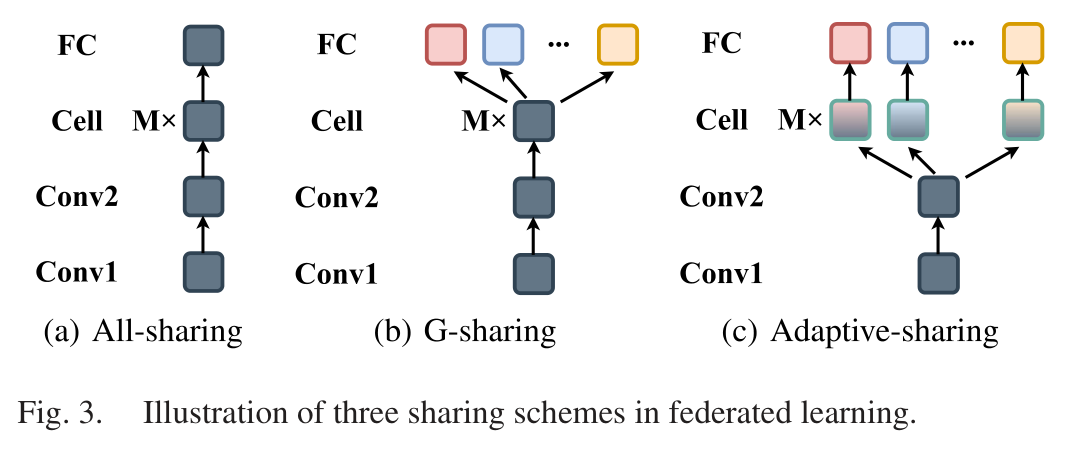
\includegraphics[width=0.98\linewidth]{figures/fig3_sharing_schemes.png}
\caption{Illustration of Three Model Sharing Schemes in Federated Learning: (a) All-Sharing, (b) $G$-Sharing, and (c) Adaptive-Sharing (FedASA).}
\label{fig:sharing_schemes}
\end{figure}

\begin{enumerate}[(a)]
    \item \textbf{All-Sharing Scheme (Figure \ref{fig:sharing_schemes}a):} Every layer of each client's neural network is transmitted to the server for aggregation. This scheme incurs immense bandwidth overhead and degrades severely when sensor locations cause feature representations to diverge.
    \item \textbf{$G$-Sharing Scheme (Figure \ref{fig:sharing_schemes}b):} Only the lowest $G$ layers of the local model are shared, while upper layers remain private. However, fixing $G$ globally across all edge devices is suboptimal because different sensor mounting coordinates require different sharing depths to balance generalization and personalization.
    \item \textbf{Adaptive-Sharing Scheme (Figure \ref{fig:sharing_schemes}c):} The proposed FedASA framework dynamically determines the optimal shared architecture depth for each device individually, adapting to each client's local dataset and bandwidth budget.
\end{enumerate}

\section{Mathematical Problem Formulation}
\enlargethispage{2\baselineskip}
Consider a federated system with an edge parameter server and $K$ heterogeneous edge devices. Each client $k \in [K] = \{1, 2, \dots, K\}$ possesses a private dataset $\mathcal{D}_k = \{(x_i^k, y_i^k)\}_{i=1}^{N_k}$. The local model is partitioned into a shared feature extractor $g_k(\cdot; \theta_k)$ and a personalized classification head $h_k(\cdot; \phi_k)$, such that the composite model is $f_k = g_k \circ h_k$.

Let $\mathcal{CO}(\theta_k^t)$ denote the uplink communication bandwidth required to transmit shared parameters $\theta_k^t$, subject to each device's communication budget $C_k$, such that $C_k^t = \mathcal{CO}(\theta_k^t) \le C_k$. To balance collective accuracy, individual resource constraints, and client equity, the multi-objective optimization problem is formulated as:
\begin{equation}
\begin{aligned}
    \min_{\{\theta_k, \phi_k\}_{k=1}^K} \quad & \sum_{k=1}^K p_k L_k(\theta_k \circ \phi_k) \\
    \text{subject to} \quad & L_k(\theta_k^T \circ \phi_k^T) - L_k(\theta_k^* \circ \phi_k^*) \le \epsilon_1, \quad \forall k \in [K] \\
    & \mathcal{CO}(\theta_k^t) \le C_k, \quad \forall k \in [K], \forall t \in [T] \\
    & \mathrm{std}\left( \left\{ L_k(\theta_k^T \circ \phi_k^T) \right\}_{k=1}^K \right) \le \epsilon_2
\end{aligned}
\end{equation}
where $\epsilon_1, \epsilon_2 > 0$ are small thresholds, $p_k = N_k / \sum_{i=1}^K N_i$, and $\mathrm{std}(\cdot)$ denotes the sample standard deviation across client losses, enforcing strict fairness across all edge devices.


%==============================================================================
% CHAPTER 4: PROPOSED METHODOLOGY
%==============================================================================
\chapter{Proposed Methodology}

The proposed FedASA (Personalized Federated Learning with Adaptive Shared Architecture) framework addresses cross-location statistical heterogeneity and device resource constraints through coordinated signal preprocessing, modular cell-based architecture design, server-side auxiliary alignment, operator-level aggregation, and confidence-aware optimization.

\section{System Architecture and Workflow Pipeline}
Figure \ref{fig:fedasa_overview} depicts the complete operational pipeline of the FedASA framework.

\begin{figure}[htbp]
\centering
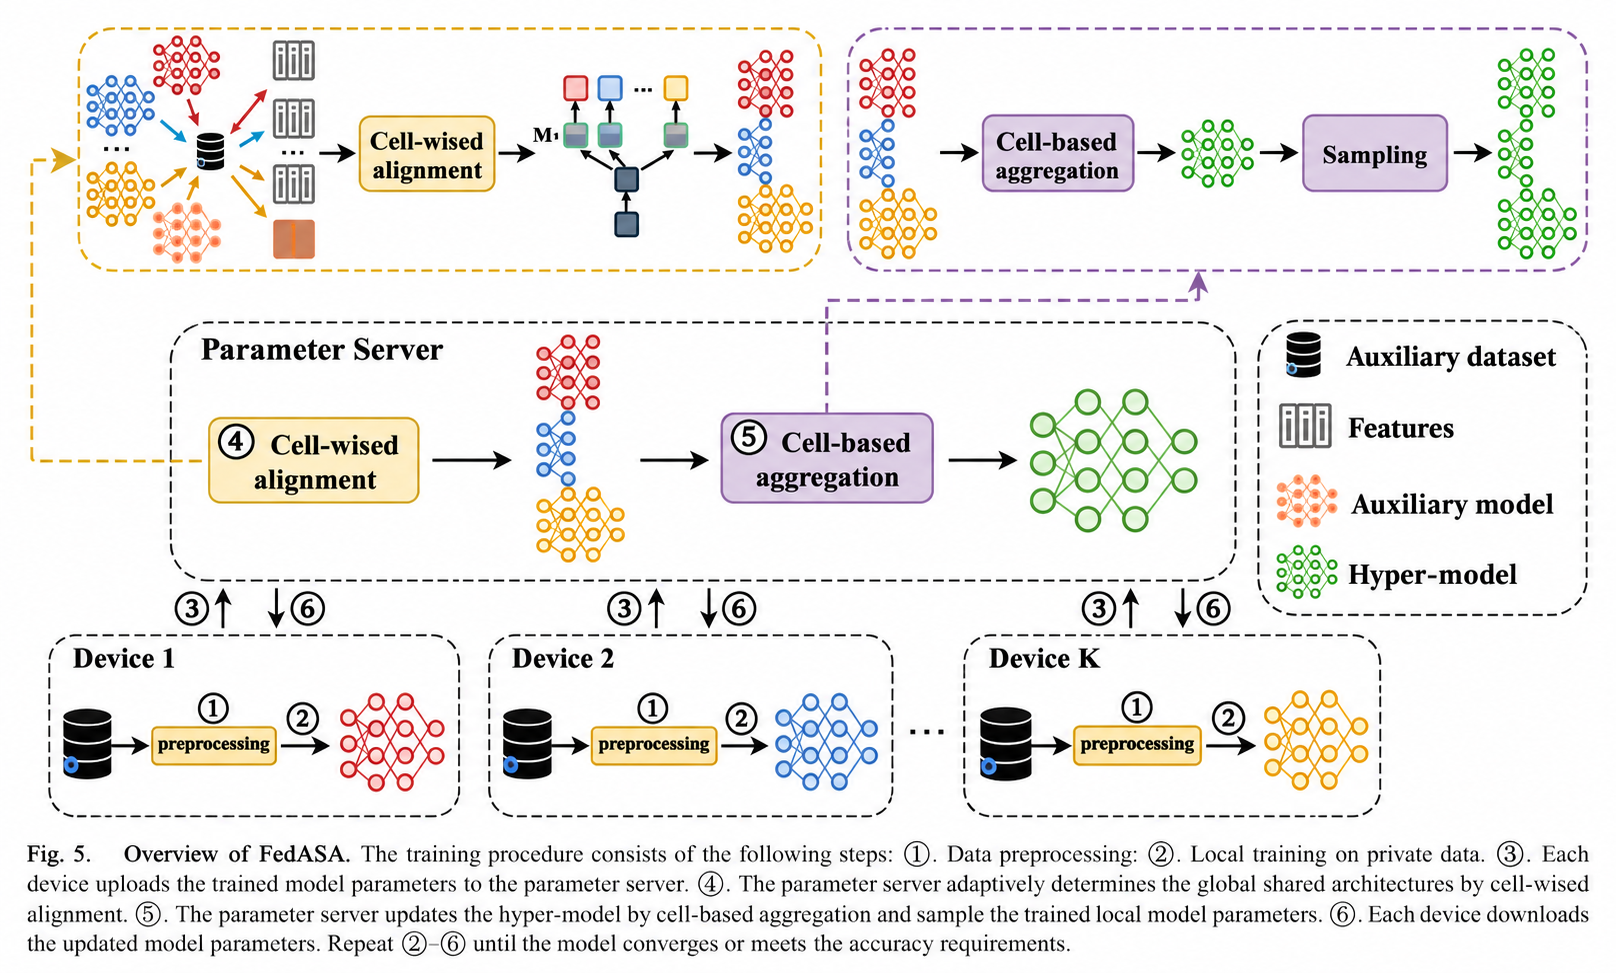
\includegraphics[width=0.98\linewidth]{figures/fig5_overview_fedasa.png}
\caption{Comprehensive Workflow Pipeline of the Proposed FedASA Framework.}
\label{fig:fedasa_overview}
\end{figure}

The training procedure executes across six sequential stages:
\begin{enumerate}
    \item \textbf{Signal Preprocessing:} Raw vibration accelerometer signals are transformed into frequency-domain spectra using Fast Fourier Transform (FFT).
    \item \textbf{Local Training:} Edge devices update their local models on private datasets using a confidence-aware hybrid loss function.
    \item \textbf{Shared Block Upload:} Edge clients transmit only their designated shared architecture blocks $\theta_k^t$ within communication budget $C_k$.
    \item \textbf{Cell-Wise Alignment:} The parameter server evaluates candidate client cells against a reference auxiliary model on an auxiliary dataset to select optimal sharing depths.
    \item \textbf{Cell-Based Aggregation:} The parameter server updates a global hyper-model by aggregating received parameters independently for each operator based on client usage frequency.
    \item \textbf{Targeted Slicing and Broadcast:} The server slices customized updated shared models from the hyper-model and broadcasts them back to each device.
\end{enumerate}

\section{Signal Preprocessing via Fast Fourier Transform (FFT)}
Raw mechanical vibration telemetry $x(t)$ represents continuous time-series data. Due to random start times and sensor mounting orientations, vibration signals collected from different machinery possess arbitrary initial phases, causing raw time-domain signals to exhibit near-zero cosine similarity ($<3\%$).

To overcome this, FedASA partitions raw signals into discrete frames of length $S = 1024$ and applies the Discrete Fourier Transform (DFT):
\begin{equation}
    X_d = \sum_{s=0}^{S-1} x_s e^{-i \frac{2\pi d s}{S}}, \quad d = 0, 1, \dots, S-1
\end{equation}
The resulting magnitude spectrum $|X_d|$ strips away arbitrary phase offsets while retaining the underlying mechanical fault frequencies and harmonic signatures, boosting cross-device feature similarity from $<3\%$ to $>85\%$.

\section{Cell-Based Modular Neural Topology}
To enable flexible partitioning without dimensional mismatch, FedASA organizes the neural network into a modular, cell-based architecture, as shown in Figure \ref{fig:model_arch}.

\begin{figure}[htbp]
\centering
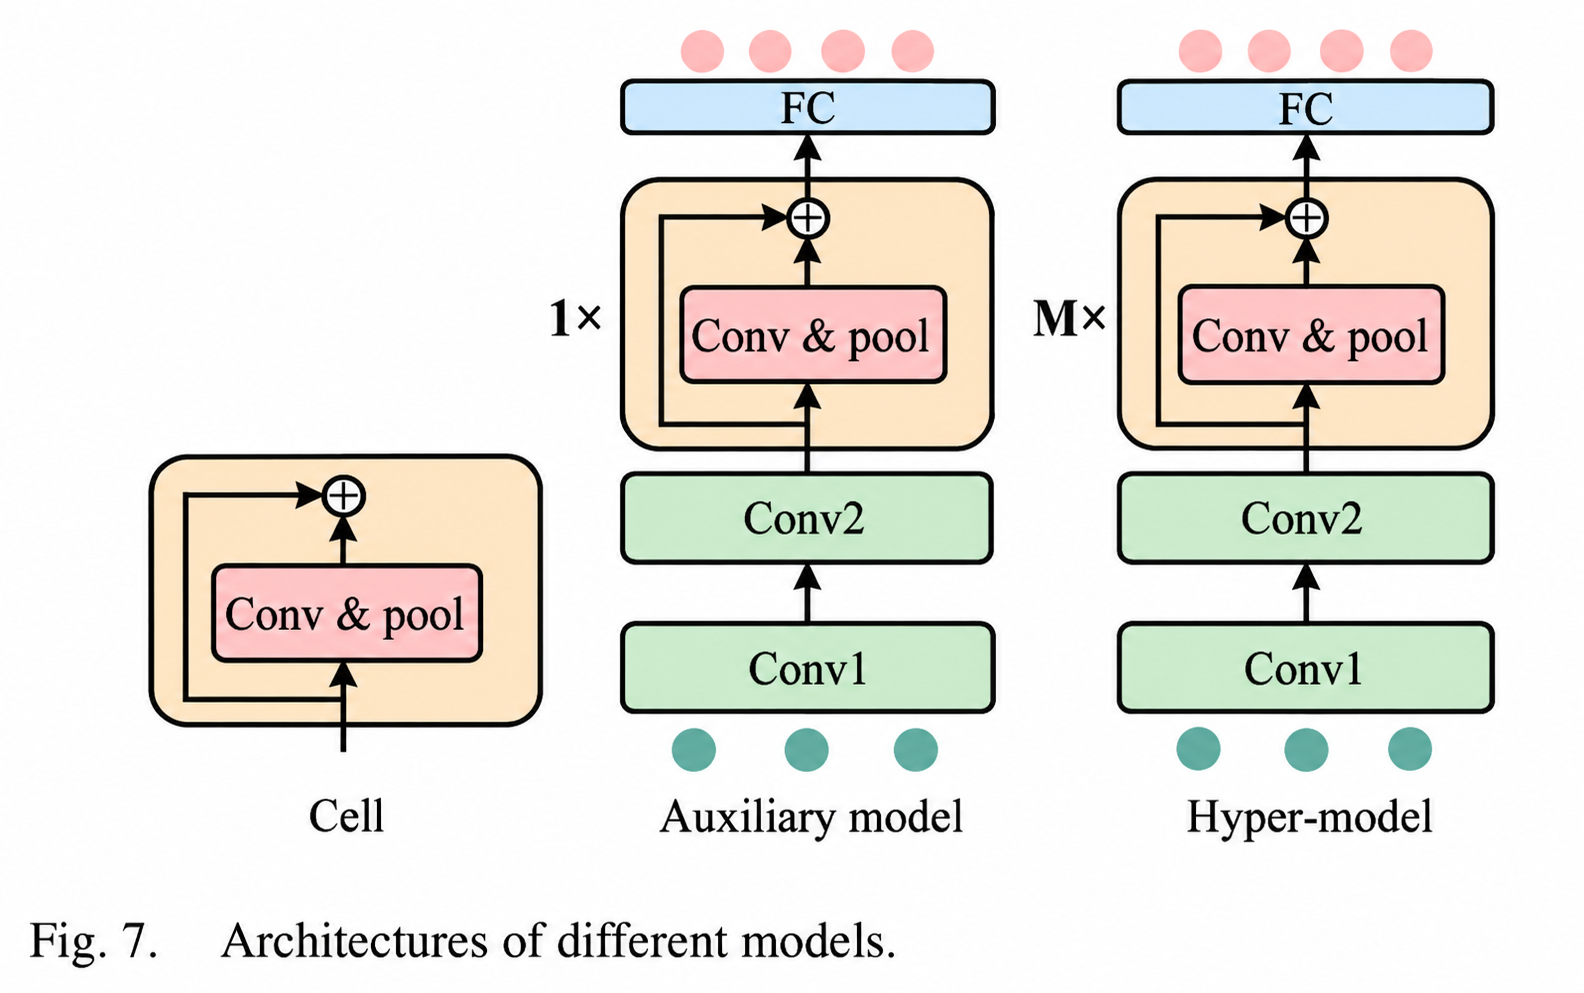
\includegraphics[width=\linewidth]{figures/fig7_model_arch.png}
\caption{Structural Architectures of the Modular Cell-Based Models: (a) Hyper-Model, (b) Auxiliary Model, and (c) Client Local Model.}
\label{fig:model_arch}
\end{figure}

Each residual cell comprises a 1D convolutional layer, batch normalization, ReLU non-linear activation, and a max-pooling operation, linked by a residual skip connection ensuring equal input and output dimensions. The composite network consists of:
\begin{itemize}
    \item An initial two-layer convolutional stem ($o_0$).
    \item A stack of $M$ identical residual cells ($o_1, \dots, o_M$).
    \item Fully connected (FC) classification layers.
\end{itemize}
Because each cell preserves feature dimensions, any prefix of $m \in [M]$ cells can seamlessly serve as the shared feature extractor $g_k^m$, while the remaining $M - m$ cells and dense layers constitute the private personalized head $h_k$.

\section{Cell-Wise Alignment Mechanism}
To determine the optimal partition depth $m_k^*$ for each device without sharing private data, the parameter server maintains an auxiliary dataset $\mathcal{D}_{\text{aux}}$ and a lightweight reference auxiliary model $g_{\text{aux}}$ containing $L$ cells ($L \le M$). The auxiliary dataset is acquired easily during initial hardware factory burn-in tests.

The server passes $\mathcal{D}_{\text{aux}}$ through candidate client sub-networks $g_k^m$ and selects the cell index $m_k^*$ that minimizes the mean squared Euclidean feature distance subject to device $k$'s communication budget:
\begin{equation}
    m_k^* = \arg\min_{m \in [M]} \mathbb{E}_{x \in \mathcal{D}_{\text{aux}}} \left\| g_{\text{aux}}^l(x; \theta_{\text{aux}}) - g_k^m(x; \theta_k) \right\|^2 \quad \text{s.t.} \quad \mathcal{CO}(\theta_k^m) \le C_k
\end{equation}
The resulting alignment vector $m^* = (m_1^*, m_2^*, \dots, m_K^*)$ governs the shared sub-network depths in subsequent training rounds.

\section{Operator-Level Cell-Based Aggregation Algorithm}
Because clients share different numbers of cells, canonical FedAvg cannot be applied directly. FedASA introduces an operator-level cell-based aggregation algorithm. Let $\mathcal{O} = \{o_0, o_1, \dots, o_M\}$ denote the structural operators. For each operator $o$, the server aggregates parameter updates only across clients that currently include operator $o$:
\begin{equation}
    \theta_{\text{hp}}^{t+1}(o) = \begin{cases}
        \sum_{k=1}^K \frac{N_{k,o}^t}{\sum_{i=1}^K N_{i,o}^t} \theta_k^t(o), & \text{if } S(o) > 0 \\
        \theta_{\text{hp}}^t(o), & \text{otherwise}
    \end{cases}
\end{equation}
where $N_{k,o}^t$ is the sample count of client $k$ sharing operator $o$, and $S(o)$ counts the number of clients sharing operator $o$ in round $t$. If all clients share operator $o$ (e.g., stem operator $o_0$), this equation reduces to FedAvg, establishing FedASA as a generalized extension of Federated Averaging.

\section{Confidence-Aware Hybrid Loss}
To resolve label ambiguity under non-IID conditions, FedASA balances soft predictions $s_i^k = \mathrm{softmax}(f_k(x_i^k))$ and hard one-hot targets $h_i^k = \mathrm{one\_hot}(\arg\max(s_i^k))$ via the predictive distribution entropy $\mathcal{E} = -\sum_{c=1}^C s_{i,c}^k \log s_{i,c}^k$:
\begin{equation}
    \hat{L}_k(\theta_k \circ \phi_k) = -\frac{1}{N_k} \sum_{i=1}^{N_k} \sum_{c=1}^C \mathbf{1}\{y_i^k = c\} \left( \log \frac{e^{s_{i,c}^k}}{\sum_{j=1}^C e^{s_{j,c}^k}} - e^{\mathcal{E}} \right)
\end{equation}
Local parameters are updated via gradient descent:
\begin{align}
    \theta_k^{t+1} &= \theta_k^t - \eta_g \nabla_{\theta} \hat{L}_k(\theta_k^t \circ \phi_k^t) \\
    \phi_k^{t+1} &= \phi_k^t - \eta_h \nabla_{\phi} \hat{L}_k(\theta_k^t \circ \phi_k^t)
\end{align}

\section{Algorithmic Execution Procedure}
Table \ref{tab:algorithm_fedasa} provides the complete algorithmic specification of FedASA.

\begin{table}[htbp]
\centering
\caption{The FedASA Algorithm Workflow}
\label{tab:algorithm_fedasa}
\vspace{0.2cm}
\begin{tabular}{|p{14.0cm}|}
\hline
\textbf{Algorithm 1: FedASA Framework} \\
\hline
\textbf{Input:} Client communication budgets $C_k$, training rounds $T$, auxiliary dataset $\mathcal{D}_{\text{aux}}$, reference model $g_{\text{aux}}$, alignment rounds $t_0$. \\
\textbf{Output:} Optimized client models $(\theta_k^T \circ \phi_k^T)$ for $k \in [K]$. \\
\textbf{Server Initialization:} Initialize hyper-model $\theta_{\text{hp}}^0$ and broadcast initial parameters. \\
\textbf{1. Server Execution (Round $t = 1, \dots, T$):} \\
\quad \textbf{if} $t \le t_0$ \textbf{then} \\
\quad \quad Receive full models $w_k^t$ from all clients $k \in [K]$. \\
\quad \quad Compute optimal cell indices: $m_k^* = \arg\min_{m \in [M]} \mathbb{E}_{\mathcal{D}_{\text{aux}}} \|g_{\text{aux}}^l - g_k^m\|^2$ s.t. $\mathcal{CO}(\theta_k^m) \le C_k$. \\
\quad \quad Construct alignment vector $m^* = (m_1^*, \dots, m_K^*)$. \\
\quad \textbf{else} \\
\quad \quad Receive shared parameter blocks $\theta_k^t(o)$ from participating devices. \\
\quad \textbf{end if} \\
\quad \textbf{for} each operator $o \in \mathcal{O}$ \textbf{do} \\
\quad \quad \textbf{if} $S(o) > 0$ \textbf{then} $\theta_{\text{hp}}^{t+1}(o) = \sum_{k=1}^K \frac{N_{k,o}^t}{\sum_{i=1}^K N_{i,o}^t} \theta_k^t(o)$ \\
\quad \quad \textbf{else} $\theta_{\text{hp}}^{t+1}(o) = \theta_{\text{hp}}^t(o)$ \\
\quad \textbf{end for} \\
\quad Slice personalized shared parameters $\theta_k^{t+1}$ using $m^*$ and broadcast to device $k$. \\
\textbf{2. Client Execution (Device $k$, Round $t = 1, \dots, T$):} \\
\quad Download updated shared parameters $\theta_k^t$ from parameter server. \\
\quad Train locally for $E$ epochs: \\
\quad \quad $\theta_k^{t+1} \leftarrow \theta_k^t - \eta_g \nabla_{\theta} \hat{L}_k(\theta_k \circ \phi_k)$ \\
\quad \quad $\phi_k^{t+1} \leftarrow \phi_k^t - \eta_h \nabla_{\phi} \hat{L}_k(\theta_k \circ \phi_k)$ \\
\quad Transmit updated shared blocks $\theta_k^{t+1}$ to parameter server. \\
\hline
\end{tabular}
\end{table}


%==============================================================================
% CHAPTER 5: THEORETICAL ANALYSIS AND GUARANTEES
%==============================================================================
\chapter{Theoretical Analysis and Guarantees}

This chapter establishes theoretical foundations for FedASA using multi-source domain adaptation theory and non-convex stochastic optimization.

\section{Multi-Source Domain Adaptation Foundations}
In classical domain adaptation (Ben-David et al. \cite{ref_bendavid_da}), let $\mathcal{D}_1$ and $\mathcal{D}_2$ denote source and target domains with error functions $L_1(f)$ and $L_2(f)$. For hypothesis space $\mathcal{F}$ with VC-dimension $d$, the target generalization error is bounded with probability at least $1-\delta$:
\begin{equation}
    L_2(f) \le L_1(f) + \frac{1}{2} \hat{d}_{\mathcal{F}\Delta\mathcal{F}}(\mathcal{D}_1, \mathcal{D}_2) + 4\sqrt{\frac{2d\log(2m) + \log(2/\delta)}{m}} + \lambda
\end{equation}
where $\hat{d}_{\mathcal{F}\Delta\mathcal{F}}$ denotes the empirical disparity difference:
\begin{equation}
    \hat{d}_{\mathcal{F}\Delta\mathcal{F}}(\mathcal{D}_1, \mathcal{D}_2) = 2 \sup_{f, f' \in \mathcal{F}} \left| \mathbb{E}_{x \sim \mathcal{D}_1} [f(x) \neq f'(x)] - \mathbb{E}_{x \sim \mathcal{D}_2} [f(x) \neq f'(x)] \right|
\end{equation}
and $\lambda = L_1(f^*) + L_2(f^*)$ is the ideal joint error constant.

\section{Federated Generalization Error Bound}
Let $\tilde{\mathcal{D}} = \sum_{k=1}^K p_k \mathcal{D}_k$ denote the fleet mixture distribution with mixture error $\tilde{L}(\cdot)$.

\noindent \textbf{Theorem 1 (Federated Error Bound):} Let $\mathcal{G}$ be the hypothesis space of shared feature extractors with VC-dimension $d$. For local sample size $m$, any $\delta \in (0,1)$, and extracted shared models $g_i \in \mathcal{G}$, the generalization error on device $i$ satisfies:
\begin{equation}
    L_i(g_i) \le \tilde{L}(g) + \frac{1}{2} \sum_{k=1}^K p_k \hat{d}_{\mathcal{G}\Delta\mathcal{G}}(\mathcal{D}_k, \mathcal{D}_i) + 4\sqrt{\frac{2d\log(2Km) + \log(2/\delta)}{Km}} + \lambda^*
\end{equation}
where $\lambda^* = \tilde{L}(g^*) + L_i(g^*)$ is the joint optimal error.

\noindent \textit{Proof:} Expanding the mixture error bound on $\sum_{k=1}^K p_k g_k$:
\begin{align}
    L_i(g_i) &\le \tilde{L}\left(\sum_{k=1}^K p_k g_k\right) + \sum_{k=1}^K p_k \left( \frac{1}{2}\hat{d}_{\mathcal{G}\Delta\mathcal{G}}(\mathcal{D}_k, \mathcal{D}_i) + \lambda_k \right) + 4\sqrt{\frac{2d\log(2Km) + \log(2/\delta)}{Km}} \nonumber \\
    &= \tilde{L}(g) + \frac{1}{2}\sum_{k=1}^K p_k \hat{d}_{\mathcal{G}\Delta\mathcal{G}}(\mathcal{D}_k, \mathcal{D}_i) + 4\sqrt{\frac{2d\log(2Km) + \log(2/\delta)}{Km}} + \sum_{k=1}^K p_k \lambda_k
\end{align}
Substituting $\sum_{k=1}^K p_k \lambda_k = \sum_{k=1}^K p_k [L_k(g^*) + L_i(g^*)] = \tilde{L}(g^*) + L_i(g^*) = \lambda^*$ completes the proof. $\blacksquare$

\section{Fairness Guarantee via Disparity Minimization}
Theorem 1 proves that client $i$'s generalization error is directly proportional to the disparity difference $\sum_{k=1}^K p_k \hat{d}_{\mathcal{G}\Delta\mathcal{G}}(\mathcal{D}_k, \mathcal{D}_i)$. By aligning candidate client representations $g_k^m$ against the common reference $g_{\text{aux}}^l$, the cell-wise alignment algorithm minimizes feature divergence, driving:
\begin{equation}
    \hat{d}_{\mathcal{G}\Delta\mathcal{G}}(\mathcal{D}_k, \mathcal{D}_i) \to 0, \quad \forall k, i \in [K]
\end{equation}
Consequently, client error bounds converge to a uniform ceiling, bounding the cross-device variance $\mathrm{std}(\{L_k\}) \le \epsilon_2$ and providing a formal mathematical guarantee of fairness.

\section{Convergence Analysis}
\noindent \textbf{Assumption 1 ($L$-Smoothness):} The global objective $L(\cdot)$ is continuously differentiable and $L$-smooth: $\|\nabla L(w_1) - \nabla L(w_2)\| \le L\|w_1 - w_2\|$, implying:
\begin{equation}
    L(w_1) - L(w_2) \le \langle \nabla L(w_2), w_1 - w_2 \rangle + \frac{L}{2}\|w_1 - w_2\|^2
\end{equation}

\noindent \textbf{Assumption 2 (Bounded Variance):} Stochastic gradients have uniformly bounded expected squared norm: $\mathbb{E}[\|\nabla \hat{L}_k(w^t)\|^2] \le G^2$ for all $k \in [K]$.

\noindent \textbf{Assumption 3 (Bounded Gradient Direction):} The aggregated direction aligns positively with the true gradient: $\nabla L(w^t)^T \mathbb{E}[\nabla \hat{L}(w^t)] \ge a \|\nabla L(w^t)\|^2$ for constant $a > 0$.

\enlargethispage{2\baselineskip}
\noindent \textbf{Lemma 1:} Under Assumption 2, the expected norm of the aggregated gradient satisfies:
\begin{equation}
    \mathbb{E}\left[ \|\nabla \hat{L}(w^t)\|^2 \right] \le K^2 G^2
\end{equation}
\noindent \textit{Proof:} By the triangle inequality and Cauchy--Schwarz:
\begin{equation}
    \|\nabla \hat{L}(w^t)\|^2 = \left\| \sum_{k=1}^K p_k \nabla \hat{L}_k(w^t) \right\|^2 \le K^2 \max_{k} \|\nabla \hat{L}_k(w^t)\|^2
\end{equation}
Taking expectations on both sides yields $\mathbb{E}[\|\nabla \hat{L}(w^t)\|^2] \le K^2 G^2$. $\blacksquare$

\noindent \textbf{Lemma 2 (One-Step Descent):} Under Assumptions 1--3, one global iteration satisfies:
\begin{equation}
    \mathbb{E}[L(w^{t+1})] \le \mathbb{E}[L(w^t)] - \eta a \mathbb{E}[\|\nabla L(w^t)\|^2] + \frac{L\eta^2 K^2 G^2}{2}
\end{equation}
\noindent \textit{Proof:} Applying $L$-smoothness with step $w^{t+1} = w^t - \eta \nabla \hat{L}(w^t)$:
\begin{equation}
    L(w^{t+1}) \le L(w^t) - \eta \nabla L(w^t)^T \nabla \hat{L}(w^t) + \frac{L\eta^2}{2}\|\nabla \hat{L}(w^t)\|^2
\end{equation}
Taking conditional expectations and substituting Assumptions 2 and 3 yields Lemma 2. $\blacksquare$

\noindent \textbf{Theorem 2 (First-Order Stationary Point Convergence):} After $T$ rounds with effective learning rate $\eta$, the average squared gradient norm satisfies:
\begin{equation}
    \frac{1}{T} \sum_{t=0}^{T-1} \mathbb{E}\left[ \| \nabla L(w^t) \|^2 \right] \le \frac{\mathbb{E}[L(w^0)] - L(w^*)}{\eta a T} + \frac{L \eta K^2 G^2}{2a}
\end{equation}
\noindent \textit{Proof:} Summing Lemma 2 from $t = 0$ to $T-1$:
\begin{equation}
    \eta a \sum_{t=0}^{T-1} \mathbb{E}[\|\nabla L(w^t)\|^2] \le \mathbb{E}[L(w^0)] - \mathbb{E}[L(w^T)] + \frac{L T \eta^2 K^2 G^2}{2}
\end{equation}
Since $\mathbb{E}[L(w^T)] \ge L(w^*)$, dividing both sides by $\eta a T$ directly yields Theorem 2. $\blacksquare$

\noindent \textbf{Remark:} Setting learning rate $\eta = \sqrt{\frac{2(\mathbb{E}[L(w^0)] - L(w^*))}{L T K^2 G^2}} = \mathcal{O}(1/\sqrt{T})$ guarantees first-order stationary point convergence at rate $\mathcal{O}(1/\sqrt{T})$.


%==============================================================================
% CHAPTER 6: PERFORMANCE EVALUATION AND RESULTS
%==============================================================================
\chapter{Performance Evaluation And Results}

This chapter details empirical evaluations on an edge prototype testbed using the Case Western Reserve University (CWRU) bearing telemetry dataset.

\section{Experimental Setup and Prototype Testbed}
Figure \ref{fig:prototype_system} illustrates the physical prototype testbed used for evaluation.

\begin{figure}[htbp]
\centering
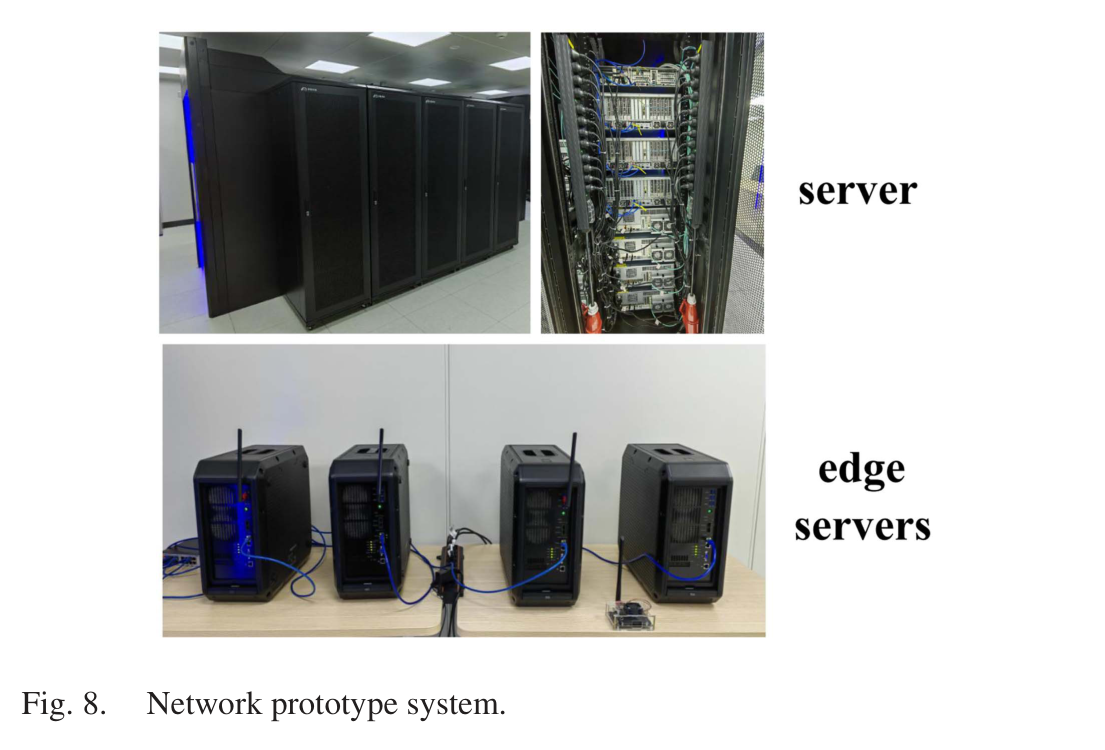
\includegraphics[width=0.88\linewidth]{figures/fig8_prototype.png}
\caption{Prototype System Architecture with Parameter Server and 4 Edge Servers Simulating 12 Distributed IoT Devices.}
\label{fig:prototype_system}
\end{figure}

The hardware configuration consists of:
\begin{itemize}
    \item \textbf{Parameter Server:} Equipped with an Intel Xeon Silver 4210R CPU @ 2.40 GHz, 64 GB DDR4 RAM, and an NVIDIA GeForce RTX 3090 GPU (Ubuntu 20.04 LTS).
    \item \textbf{Edge Servers:} Four networked edge servers, each hosting three isolated virtual environments to simulate 12 distributed IoT edge clients.
    \item \textbf{Software Framework:} PyTorch 1.12.0 with CUDA 11.6 acceleration.
\end{itemize}

\section{Benchmark Dataset Description}
Evaluations utilized the rolling element bearing dataset from the Case Western Reserve University (CWRU) bearing data center \cite{ref_cwru_dataset}. Telemetry signals were acquired from vibration sensors mounted at three physical locations:
\begin{itemize}
    \item \textbf{Location A (Drive-End):} Accelerometer mounted at the drive-end of the motor housing.
    \item \textbf{Location B (Fan-End):} Accelerometer placed at the motor fan-end housing.
    \item \textbf{Location C (Base Plate):} Accelerometer positioned on the machine base plate supporting the apparatus.
\end{itemize}

Four distinct bearing operating conditions were evaluated: Normal baseline (N), Inner Race defect (IR), Ball defect (BR), and Outer Race defect (OR). Defect diameters measured 7, 14, and 21 mils, producing 10 mutually exclusive classification states. Table \ref{tab:cwru_dataset} provides the dataset parameters.

\begin{table}[htbp]
\centering
\caption{Structural Description of the CWRU Bearing Fault Dataset}
\label{tab:cwru_dataset}
\vspace{0.2cm}
\resizebox{\linewidth}{!}{
\begin{tabular}{|l|c|c|c|}
\hline
\textbf{Bearing Health State} & \textbf{Defect Diameter (mils)} & \textbf{Sensor Locations} & \textbf{Class Labels} \\
\hline
Normal State (N) & Nil & A, B, C & Class 0 \\
Inner Race Fault (IR) & 7, 14, 21 & A, B, C & Classes 1, 2, 3 \\
Ball Fault (BR) & 7, 14, 21 & A, B, C & Classes 4, 5, 6 \\
Outer Race Fault (OR) & 7, 14, 21 & A, B, C & Classes 7, 8, 9 \\
\hline
\end{tabular}
}
\end{table}

The 12 simulated devices were assigned tasks spanning 4 mechanical loads (0, 1, 2, 3 HP) across the three monitoring coordinates, as summarized in Table \ref{tab:device_allocation}.

\begin{table}[htbp]
\centering
\caption{Device Task and Location Configuration}
\label{tab:device_allocation}
\vspace{0.2cm}
\resizebox{\linewidth}{!}{
\begin{tabular}{|c|c|c|c|c|}
\hline
\textbf{Device ID} & \textbf{Sensor Location} & \textbf{Motor Load (HP)} & \textbf{Speed (RPM)} & \textbf{Samples (Train / Test)} \\
\hline
Dev 1 -- 4 & Drive-End (A) & 0, 1, 2, 3 & 1797, 1772, 1750, 1730 & 800 / 200 per device \\
Dev 5 -- 8 & Fan-End (B) & 0, 1, 2, 3 & 1797, 1772, 1750, 1730 & 800 / 200 per device \\
Dev 9 -- 12 & Base Plate (C) & 0, 1, 2, 3 & 1797, 1772, 1750, 1730 & 800 / 200 per device \\
\hline
\end{tabular}
}
\end{table}

\section{Diagnostic Accuracy Across Sensor Locations}
Table \ref{tab:diagnostic_accuracy} reports the classification accuracy and standard deviation across four cross-location configurations.

\begin{table}[htbp]
\centering
\caption{Diagnostic Accuracy (\%) and Standard Deviation across Sensor Mounting Locations}
\label{tab:diagnostic_accuracy}
\vspace{0.2cm}
\resizebox{\linewidth}{!}{
\begin{tabular}{|l|c|c|c|c|}
\hline
\textbf{Method} & \textbf{Locations A \& B} & \textbf{Locations A \& C} & \textbf{Locations B \& C} & \textbf{Locations A, B \& C} \\
\hline
Local-Only & $58.12 \pm 6.45$ & $52.34 \pm 7.12$ & $61.40 \pm 5.89$ & $51.78 \pm 8.24$ \\
FedAvg \cite{ref_mcmahan_fedavg} & $82.45 \pm 5.12$ & $74.60 \pm 6.30$ & $88.15 \pm 4.20$ & $70.22 \pm 6.78$ \\
FedProx \cite{ref_li_fedprox} & $81.13 \pm 4.90$ & $72.50 \pm 5.80$ & $86.67 \pm 3.95$ & $68.92 \pm 6.15$ \\
Ditto \cite{ref_li_ditto} & $89.50 \pm 3.40$ & $83.25 \pm 4.10$ & $91.80 \pm 2.85$ & $84.17 \pm 3.90$ \\
FedPer \cite{ref_arivazhagan_fedper} & $93.10 \pm 2.80$ & $88.40 \pm 3.65$ & $94.50 \pm 2.15$ & $91.42 \pm 3.10$ \\
\hline
\textbf{FedASA (Ours)} & $\mathbf{97.20 \pm 1.45}$ & $\mathbf{96.15 \pm 1.80}$ & $\mathbf{98.10 \pm 1.10}$ & $\mathbf{97.44 \pm 1.25}$ \\
\hline
\end{tabular}
}
\end{table}

Key performance observations include:
\begin{itemize}
    \item \textbf{Superior Tri-Location Diagnostic Accuracy:} Under the most challenging scenario where clients are distributed across all three mounting coordinates (A, B \& C), FedASA attains \textbf{97.44\%} diagnostic accuracy, outperforming canonical FedAvg ($70.22\%$) by \textbf{27.22\%} and state-of-the-art FedPer ($91.42\%$) by \textbf{6.02\%}.
    \item \textbf{Robustness across Dissimilar Sensor Pairs:} When evaluating Locations A \& C-the pair exhibiting the lowest cosine similarity ($58.4\%$)-FedProx suffers an accuracy drop down to $72.50\%$, whereas FedASA maintains an accuracy of \textbf{96.15\%}.
\end{itemize}

\section{Communication Bandwidth Savings}
Figure \ref{fig:bandwidth_savings} compares the uplink communication requirement per client per training round.

\begin{figure}[htbp]
\centering
\resizebox{0.90\textwidth}{!}{
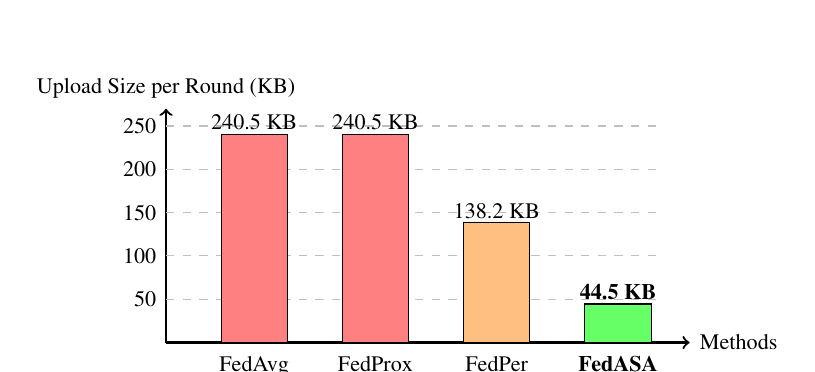
\begin{tikzpicture}[xscale=0.7, yscale=0.011]
    \draw[->, thick] (0,0) -- (9.5,0) node[right] {\footnotesize Methods};
    \draw[->, thick] (0,0) -- (0,270) node[above] {\footnotesize Upload Size per Round (KB)};

    \draw[dashed, color=gray!50] (0,50) -- (9,50) node[left, color=black] at (0,50) {\footnotesize 50};
    \draw[dashed, color=gray!50] (0,100) -- (9,100) node[left, color=black] at (0,100) {\footnotesize 100};
    \draw[dashed, color=gray!50] (0,150) -- (9,150) node[left, color=black] at (0,150) {\footnotesize 150};
    \draw[dashed, color=gray!50] (0,200) -- (9,200) node[left, color=black] at (0,200) {\footnotesize 200};
    \draw[dashed, color=gray!50] (0,250) -- (9,250) node[left, color=black] at (0,250) {\footnotesize 250};

    \draw[fill=red!50, draw=black] (1,0) rectangle (2.2,240.5);
    \node at (1.6,255) {\footnotesize 240.5 KB};
    \node[below] at (1.6,-5) {\footnotesize FedAvg};

    \draw[fill=red!50, draw=black] (3.2,0) rectangle (4.4,240.5);
    \node at (3.8,255) {\footnotesize 240.5 KB};
    \node[below] at (3.8,-5) {\footnotesize FedProx};

    \draw[fill=orange!50, draw=black] (5.4,0) rectangle (6.6,138.2);
    \node at (6.0,152) {\footnotesize 138.2 KB};
    \node[below] at (6.0,-5) {\footnotesize FedPer};

    \draw[fill=green!60, draw=black] (7.6,0) rectangle (8.8,44.5);
    \node at (8.2,58) {\footnotesize \textbf{44.5 KB}};
    \node[below] at (8.2,-5) {\footnotesize \textbf{FedASA}};
\end{tikzpicture}
}
\caption{Uplink Communication Payload per Client per Training Round.}
\label{fig:bandwidth_savings}
\end{figure}

Monolithic all-sharing schemes (FedAvg, FedProx) require transmitting $240.5\text{ KB}$ per round. FedPer transmits $138.2\text{ KB}$ by reserving upper classification layers locally. In contrast, FedASA transmits between $10.46\text{ KB}$ and $59.87\text{ KB}$ (averaging \textbf{44.5 KB}), achieving an overall bandwidth reduction of \textbf{81.49\%}.

\enlargethispage{1.5\baselineskip}
\section{Client Fairness and Convergence Acceleration}
Across all evaluated configurations, FedASA maintained an accuracy standard deviation below $\mathbf{1.80\%}$ (compared to $\pm 8.24\%$ for local training and $\pm 6.78\%$ for FedAvg). This confirms that edge clients achieve uniform predictive accuracy regardless of whether their sensors are mounted at primary drive-end locations or peripheral base plates.

Furthermore, FedASA achieves $>95\%$ accuracy within \textbf{80 communication rounds}, accelerating convergence by more than $2.5\times$ compared to Ditto and FedPer ($>200$ rounds).

\section{Ablation Study and Hyperparameter Sensitivity}
Figure \ref{fig:ablation_arch} evaluates the impact of fixed sharing schemes versus adaptive selection, and Figure \ref{fig:hyperparam} examines sensitivity to auxiliary model depth $l$.

Key findings include:
\begin{itemize}
    \item \textbf{Suboptimality of Fixed Partitions:} In Locations A \& B, the optimal static partition $\alpha_1$ achieves $96.33\%$, while $\alpha_4$ drops to $90.88\%$ (a $5.45\%$ discrepancy). Static sharing cannot satisfy divergent cross-location demands.
    \item \textbf{Low Sensitivity to Auxiliary Depth:} Varying auxiliary model cell depth $l$ from 0 to 4 alters accuracy by less than $1.29\%$. Even a modest auxiliary model with $78.12\%$ accuracy provides sufficient guidance for robust cell-wise alignment.
\end{itemize}

\begin{figure}[p]
\centering
\vspace*{-10pt}
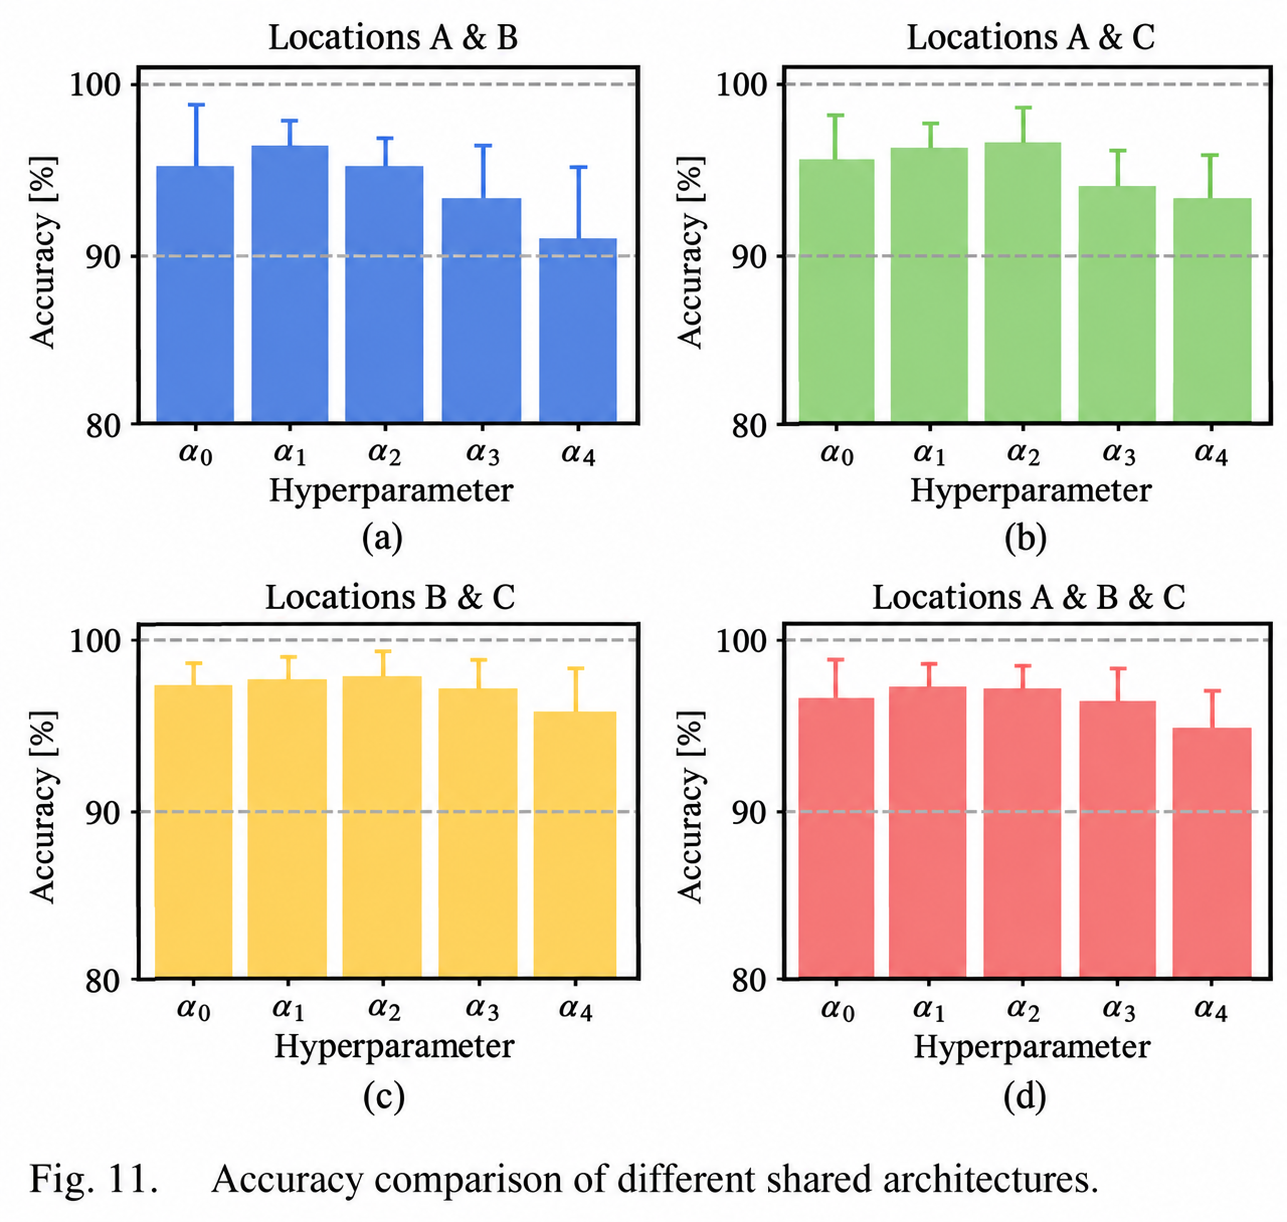
\includegraphics[width=0.78\linewidth]{figures/fig11_shared_arch.png}
\caption{Accuracy Comparison across Fixed Shared Architectures ($\alpha_0$ to $\alpha_4$).}
\label{fig:ablation_arch}
\vspace{0.3cm}
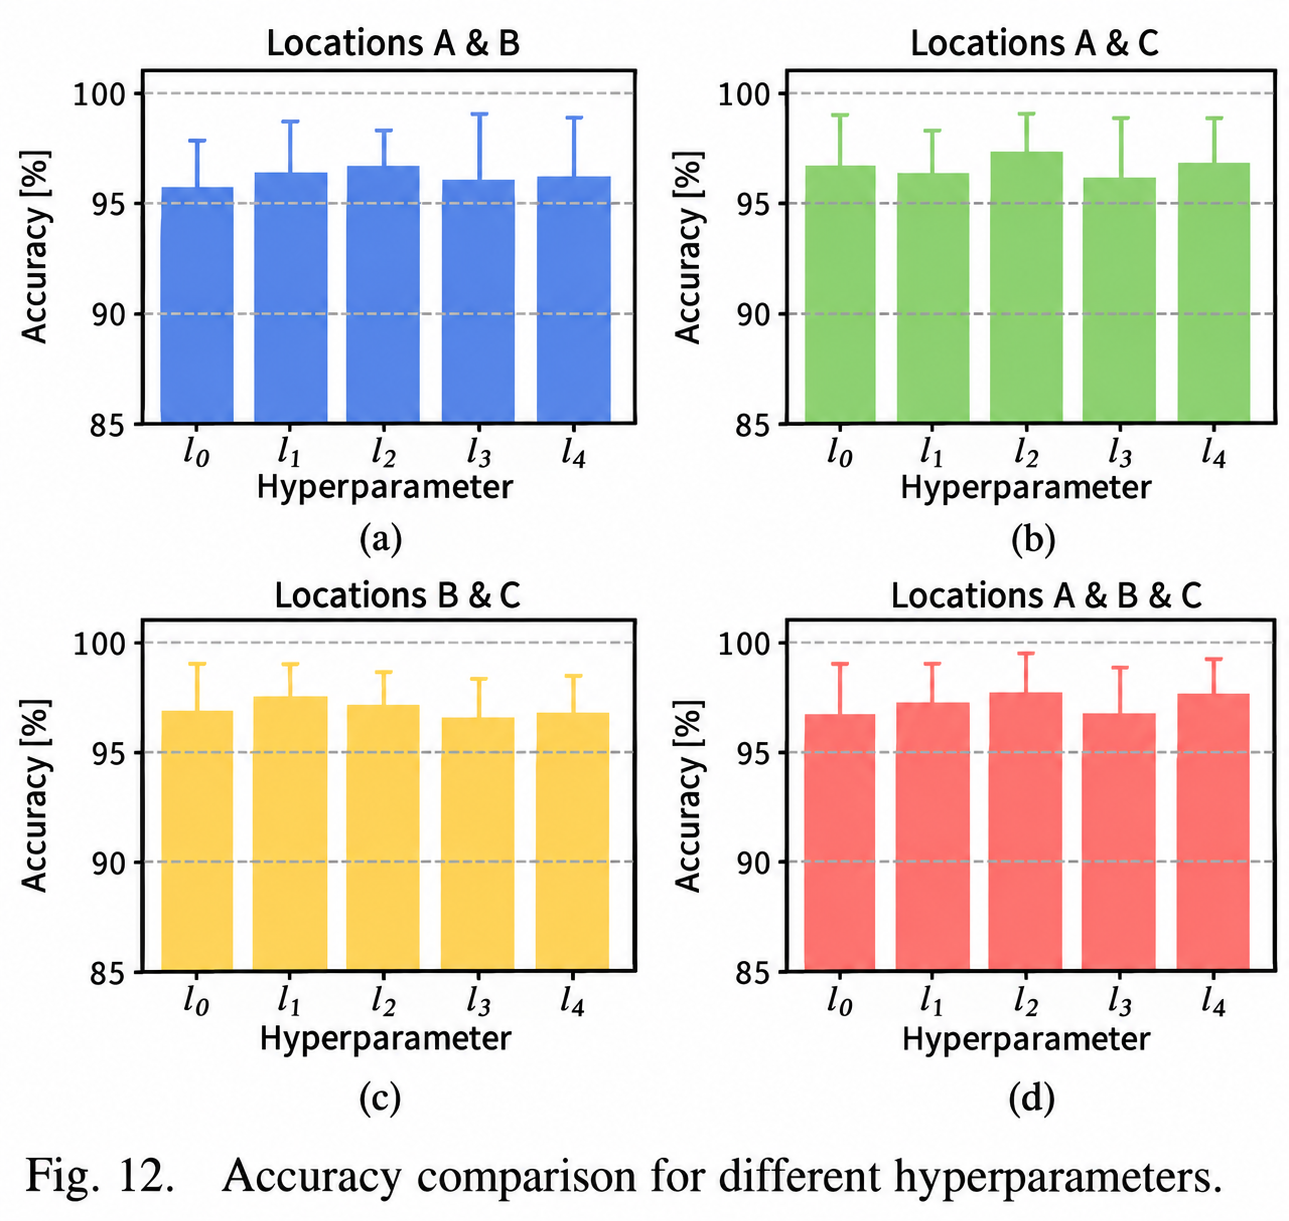
\includegraphics[width=0.78\linewidth]{figures/fig12_hyperparams.png}
\caption{Impact of Auxiliary Model Depth ($l = 0, 1, 2, 3, 4$) on Diagnostic Accuracy.}
\label{fig:hyperparam}
\end{figure}

\section{Feature Representation Visualization}
To investigate feature representations learned by FedASA, high-dimensional representations were projected onto a 2D manifold using t-SNE \cite{ref_tsne}, as shown in Figure \ref{fig:tsne_viz}.

\begin{figure}[htbp]
\centering
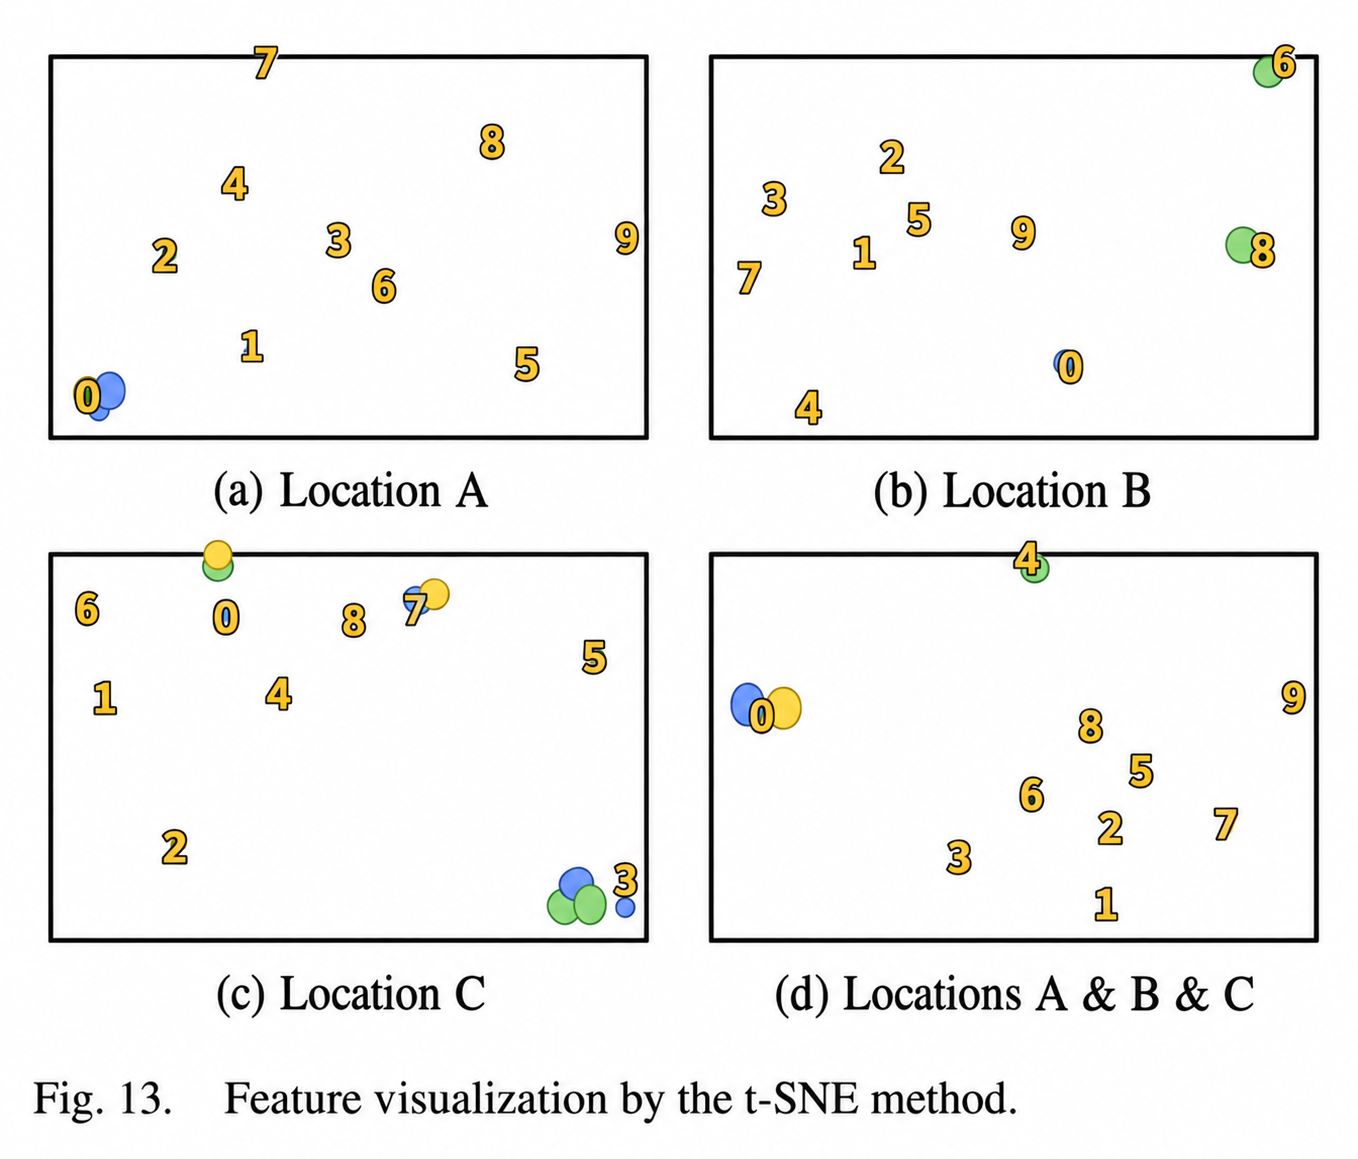
\includegraphics[width=0.88\linewidth]{figures/fig13_tsne.png}
\caption{Two-Dimensional t-SNE Feature Representation Visualization of Bearing Fault Classes under the FedASA Framework.}
\label{fig:tsne_viz}
\end{figure}

The visualization reveals clean, well-separated cluster margins among all 10 bearing fault classes without cross-class intermingling, corroborating the high diagnostic accuracy.


%==============================================================================
% CHAPTER 7: CONCLUSION AND FUTURE SCOPE
%==============================================================================
\chapter{Conclusion}

This seminar presented an in-depth investigation of \textbf{FedASA}, a personalized federated learning framework with adaptive model aggregation designed for resource-constrained Mobile Edge Computing and Industrial IoT environments. 

\section{Summary of Contributions}
The key contributions discussed in this report are:
\begin{enumerate}
    \item \textbf{Identification of the Cross-Location Challenge:} Demonstrated that differing physical sensor mounting coordinates induce substantially more severe statistical heterogeneity ($<58.4\%$ cosine similarity) than machinery operational condition shifts ($>87.5\%$), triggering severe performance degradation in conventional FL.
    \item \textbf{Adaptive Cell-Wise Alignment:} Introduced an auxiliary alignment mechanism on the parameter server that dynamically customizes the boundary between shared and personalized layers for each client under communication constraints.
    \item \textbf{Operator-Level Modular Aggregation:} Formulated a cell-based aggregation algorithm that updates global hyper-model parameters based on operator usage frequency, strictly generalizing Federated Averaging.
    \item \textbf{Rigorous Theoretical Guarantees:} Established domain-adaptation generalization error bounds proving strict client fairness and proved first-order stationary point convergence at rate $\mathcal{O}(1/\sqrt{T})$.
    \item \textbf{Empirical Superiority:} Benchmark validation on the CWRU dataset demonstrated \textbf{97.44\% diagnostic accuracy} (outperforming FedAvg by $27.22\%$), up to \textbf{81.49\% communication bandwidth savings}, and low accuracy variance ($<1.80\%$).
\end{enumerate}

\section{Limitations and Practical Deployment Challenges}
Despite its significant advantages, deploying FedASA in industrial practice faces specific limitations:
\begin{itemize}
    \item \textbf{Auxiliary Dataset Requirement:} The server relies on a representative auxiliary dataset to align client features. While factory burn-in data can provide this, unmodeled environmental noise may affect alignment accuracy.
    \item \textbf{Synchronous Round Assumptions:} The current framework assumes synchronized client rounds, which may encounter straggler delays in unreliable industrial wireless networks.
\end{itemize}

\section{Future Research Directions}
Promising future research avenues include:
\begin{itemize}
    \item \textbf{Asynchronous Client Aggregation:} Developing asynchronous aggregation extensions to accommodate device intermittent availability and lossy wireless channels.
    \item \textbf{Extreme Dirichlet Label Skew:} Extending adaptive cell alignment to handle severe pathological label imbalance alongside spatial sensor heterogeneity.
    \item \textbf{Differential Privacy Integration:} Incorporating differentially private perturbation mechanisms into auxiliary alignment feature exchanges to protect server-side auxiliary datasets.
    \item \textbf{Multi-Modal Sensor Telemetry Fusion:} Extending modular cell architectures to fuse heterogeneous multi-modal inputs, including high-frequency acoustic emissions, motor current signatures, and thermal infrared imaging.
\end{itemize}


%==============================================================================
% REFERENCES
%==============================================================================
\begin{thebibliography}{99}
\addcontentsline{toc}{chapter}{References}
\sloppy

\bibitem{ref_fedasa}
D.~Deng, X.~Wu, T.~Zhang, X.~Tang, H.~Du, J.~Kang, J.~Liu, and D.~Niyato, ``FedASA: A personalized federated learning with adaptive model aggregation for heterogeneous mobile edge computing,'' \textit{IEEE Transactions on Mobile Computing}, vol.~23, no.~11, pp.~10842--10857, Nov.~2024.

\bibitem{ref_mcmahan_fedavg}
B.~McMahan, E.~Moore, D.~Ramage, S.~Hampson, and B.~A.~y~Arcas, ``Communication-efficient learning of deep networks from decentralized data,'' in \textit{Proceedings of the 20th International Conference on Artificial Intelligence and Statistics (AISTATS)}, 2017, pp.~1273--1282.

\bibitem{ref_li_fedprox}
T.~Li, A.~K.~Sahu, M.~Sanjabi, and V.~Smith, ``Federated optimization in heterogeneous networks,'' in \textit{Proceedings of Machine Learning and Systems (MLSys)}, vol.~2, 2020, pp.~429--450.

\bibitem{ref_li_ditto}
T.~Li, S.~Hu, A.~Beirami, and V.~Smith, ``Ditto: Fair and robust federated learning through personalization,'' in \textit{Proceedings of the 38th International Conference on Machine Learning (ICML)}, 2021, pp.~6357--6368.

\bibitem{ref_arivazhagan_fedper}
M.~G.~Arivazhagan and V.~Aggarwal, ``Federated learning with personalization layers,'' \textit{arXiv preprint arXiv:1912.00818}, 2019.

\bibitem{ref_collins_fedrep}
L.~Collins, H.~Hassani, A.~Mokhtari, and S.~Shakkottai, ``Exploiting shared representations for personalized federated learning,'' in \textit{Proceedings of the 38th International Conference on Machine Learning (ICML)}, 2021, pp.~2089--2099.

\bibitem{ref_fallah_perfedavg}
A.~Fallah, A.~Mokhtari, and A.~Ozdaglar, ``Personalized federated learning with theoretical guarantees: A model-agnostic meta-learning approach,'' in \textit{Advances in Neural Information Processing Systems (NeurIPS)}, vol.~33, 2020, pp.~3557--3568.

\bibitem{ref_cwru_dataset}
W.~A.~Smith and R.~B.~Randall, ``Rolling element bearing diagnostics using the Case Western Reserve University data: A benchmark study,'' \textit{Mechanical Systems and Signal Processing}, vol.~64, pp.~100--131, 2015.

\bibitem{ref_bendavid_da}
S.~Ben-David, J.~Blitzer, K.~Crammer, A.~Kulesza, F.~Pereira, and J.~W.~Vaughan, ``A theory of learning from different domains,'' \textit{Machine Learning}, vol.~79, no.~1, pp.~151--175, 2010.

\bibitem{ref_tsne}
L.~van~der~Maaten and G.~Hinton, ``Visualizing data using t-SNE,'' \textit{Journal of Machine Learning Research}, vol.~9, no.~11, pp.~2579--2605, 2008.

\bibitem{ref_zhao_datasharing}
Y.~Zhao, M.~Li, L.~Lai, N.~Suda, D.~Civin, and V.~Chandra, ``Federated learning with non-IID data,'' \textit{arXiv preprint arXiv:1806.00582}, 2018.

\bibitem{ref_fedgen}
Z.~Zhu, J.~Hong, and J.~Zhou, ``Data-free knowledge distillation for heterogeneous federated learning,'' in \textit{Proceedings of the 38th International Conference on Machine Learning (ICML)}, 2021, pp.~12878--12889.

\bibitem{ref_fedftg}
C.~Zhang, K.~Shen, and L.~Gao, ``FedFTG: Fine-tuning global model with generative knowledge distillation for heterogeneous federated learning,'' \textit{arXiv preprint arXiv:2208.11292}, 2022.

\bibitem{ref_qiu_edge_iiot}
T.~Qiu, J.~Chi, X.~Zhou, Z.~Ning, M.~Atiquzzaman, and D.~O.~Wu, ``Edge computing in industrial Internet of Things: Architecture, advances and challenges,'' \textit{IEEE Communications Surveys \& Tutorials}, vol.~22, no.~4, pp.~2462--2488, 2020.

\bibitem{ref_regatti_fedcma}
J.~R.~Regatti, G.~Gupta, A.~Koushik, and A.~Gopalan, ``FedCMA: Conditional model alignment for improved generalization in federated learning,'' in \textit{Proceedings of the International Conference on Neural Information Processing Systems (NeurIPS)}, 2022.

\end{thebibliography}

\end{document}
